\documentclass[11pt,a4paper]{article}
\usepackage[utf8]{inputenc}
\usepackage{amsmath}
\usepackage{amsfonts}
\usepackage{amssymb}
\usepackage{graphicx}
\usepackage[margin=0.6in]{geometry}
\usepackage{lipsum}
\usepackage{rotating}
\usepackage{epstopdf}
\usepackage[numbers]{natbib}
\usepackage[toc,page]{appendix}
\usepackage{subcaption}
\usepackage[section]{placeins}
\usepackage{pdfpages}
\usepackage{afterpage}

\newcommand\blankpage{%
    \null
    \thispagestyle{empty}%
    \addtocounter{page}{-1}%
    \newpage}

\newcommand{\q}[1]{``#1''}

\author{Bilhal Salhani Maat, Jan}

\title{Proton Computed Tomography and Image Reconstruction}
\date{March 15, 2016}
\author{Bilhal Salhani Maat}

\begin{document}

\includepdf[pages={1}]{kthcover.pdf}
\blankpage

\begin{titlepage}
    \begin{center}
        \vspace*{0.5cm}
        \LARGE
        %\textbf{Proton Computed Tomography\\and\\Image Reconstruction}
        \textbf{Backprojection-then-filtering reconstruction \\along the most likely path \\in proton computed tomography\\}
        \vspace{0.5cm}
        \LARGE
		Master Thesis
        
        \vspace{1.cm}
        
        \textbf{Bilhal Salhani Maat}
        \vspace{0.7cm}
        \abstract{The backprojection-then-filtering algorithm was applied to proton CT data to reconstruct a map of proton stopping power relative to water (RSP) in air, water and bone. Backprojections were performed along three commonly used path estimates for the proton: straight line path, cubic spline path, and most likely path. The proton CT data was obtained through simulations using the GEANT4 simulation toolkit. Two elliptical phantoms were inspected, and an accuracy of 0.2\% and 0.8\% was obtained for the RSP in water and bone respectively in the region of interest, while the RSP of air was significantly underestimated.}
        
        %The abstract will go here to talk about the backprojection then filtering algorithm, the most likely path, and the attempt to do it for more materials like bone and air (and maybe others if I have time). And comparing cubic spline resolution to most likely path resolution of images.}
        \vspace{0.7cm}
        
        %Literature review
        
        %\vspace{0.8cm}
        \centering
        \includegraphics[width=0.4\textwidth]{img/kthlogo.png}\\
        \vspace{1.0cm}
        \includegraphics[width=0.4\textwidth]{img/manchesterlogo.png}
        
        \vspace{0.8cm}
		\large
        School of Medical Engineering\\
        KTH University, Sweden\\
        \&\\
        PRECISE group,\\
        University of Manchester, UK\\
        May 27, 2016
        
    \end{center}
    \textbf{Supervisor:} Dr. Michael Merchant
\end{titlepage}

%{\centering \includegraphics[scale=0.35]{kthlogo.png}\\}
{\let\newpage\relax}


%\abstract{The abstract will go here to talk about the backprojection then filtering algorithm, the most likely path, and the attempt to do it for more materials like bone and air (and maybe others if I have time). And comparing cubic spline resolution to most likely path resolution of images.}

\tableofcontents
\newpage
\section{Introduction}
In recent years there has been rapid proliferation in the number of proton therapy centres worldwide. At the time of writing, there are 56 centres worldwide in operation and 30 centres under construction \cite{ptcog}. The recent surge in interest in proton therapy is in large part due to the technological advances of the last three decades brought about by the particle physics community. The advantageous characteristics of proton energy deposition and its application in radiotherapy has long been known \cite{wilson1946radiological} and the first patient to undergo hospital-based proton therapy was treated with protons for ocular melanoma in 1991 at the Loma Linda University Medical Centre in the United States \cite{schulte2012new}. Until recently, however, the cost-to-benefit ratio relative to conventional radiotherapy was not enough to warrant the construction of large and expensive proton beam facilities.

The biggest advantage of proton therapy over traditional forms of radiotherapy exhibits itself in the form of the Bragg peak, a consequence of the way in which protons deposit energy as they traverse a medium (see figure \ref{fig:braggpeak} in appendix \ref{app:intro}). Due to the low dose deposition of protons up until the Bragg peak, and their steep depth-dose fall off at the distal end of the Bragg peak, protons are theoretically able to provide a more conformal dose distribution to a tumour volume while minimizing dose to normal tissue and sparing critical normal structures. This is of particular importance when irradiating tumour volumes in the central nervous system and near organs sensitive to radiation, and in children who are at high risk of developing secondary cancers.

%\subsection{Uncertainties associated with proton therapy}
Theoretically, proton therapy promises more conformal dose distributions and lesser doses to healthy tissue. However, this is under the assumption that an ideal treatment plan can be implemented and uncertainties at the time of treatment are minimised. In reality, as with other forms of therapy, there are various sources of errors in both the treatment planning stage and during irradiation \cite{erdelyi2011some,knopf2013vivo}. Errors can stem from proton range uncertainties caused by material heterogeneity, and from organ deformation and internal motion between the planning and treatment stages. Furthermore, the patient position as planned during the planning stage must be reproduced in the treatment room. Set up errors can lead to slight changes in the distribution of tissues relative to the beam, and interfractional changes in patients, such as weight changes or tumour shrinkage, can also result in further uncertainties. Treatment planning systems can also result in uncertainties in the dose deposition to the patient due to inaccurate models of nuclear interactions.

One of the potential sources of error is the estimation of the stopping power of protons relative to water (RSP) in a medium \cite{yang2012comprehensive}. Proton computed tomography (pCT) (see appendix \ref{sec:pCT}), a new imaging modality, is currently being investigated and has the potential to provide better estimates of RSP compared to conventional methods by directly measuring the RSP using protons. Proton computed tomography and the application of filtered backprojection and backprojection then filtering image reconstruction algorithms applied to pCT data are the subject of this thesis.

%This is particularly relevant when using protons as uncertainties can lead to high doses being deposited at critical structures.


%Talk about motivation by proton CT. Number of proton therapy facilities in world. Problems associated with it. Goal of project - investigating FBP reconstruction methods in proton CT.

\subsection{Proton therapy treatment planning}

Current proton therapy treatment plans are determined using images acquired through traditional x-ray CT some time prior to a patient's first treatment. X-ray CT scans measure the photon attenuation coefficients of a medium which are then converted to Hounsfield units (HU)\footnote{The HU values are a linear transformation of the photon attenuation coefficients obtained through x-ray CT, $\mu$, where $HU = 1000 \times (\mu - \mu_{water})/(\mu_{water} - \mu_{air})$, where $\mu_{air}$ and $\mu_{water}$ are the photon attenuation coefficients of air and water respectively.}. The RSP can then be obtained through a predetermined relationship between HU and RSP. The predetermined relationship, known as a calibration curve, is unique and must be calculated for each CT scanner \cite{constantinou1992electron}. 

The simplest method of determining the calibration curve relies on the use of tissue equivalent substitutes of known density and elemental composition. By measuring the HU and RSP of various tissue equivalent substitutes, one can arrive at a relationship between HU and RSP. However, due to the fact that the tissue equivalent substitutes are not truly equivalent to human tissue, calibration curves obtained in this way are sensitive to the tissue substitutes used. It is for this reason that Schneider et al proposed the stoichiometric method \cite{schneider1996calibration}, which was shown to be less sensitive to the tissue substitutes used in the calibration. However, this method still suffers from a degeneracy problem - there does not exist a one-to-one correspondence between HU and RSP, and tissues with the same HU can have different RSP. An investigation into the uncertainties associated with RSPs obtained using the stoichiometric method has been studied in \cite{yang2012comprehensive}, and the variation in RSP due to differences in tissue composition has been investigated by Yang et al \cite{yang2010theoretical}. 

During treatment, in vivo range verification of the proton beam can be carried out using a multitude of methods, including implantable dosimeters, prompt gamma imaging, and positron emission tomography \cite{knopf2013vivo}, each with their own advantages and limitations. 

This project addresses the issue of pretreatment planning and the distribution of tissues within an area being irradiated. Proton computed tomography is able to overcome the uncertainties associated with the conversion from HU to RSP by directly measuring RSP (see appendix \ref{sec:WEPL}). Furthermore, if one was able to use protons at the pretreatment stage in the treatment room, uncertainties due to patient set up can be further minimised (current pretreatment imaging is performed using x-ray cone beam CT).

\subsection{Proton detector technology}
\label{sec:detector}
The accuracy of the maps of RSP obtained through pCT are dependent on both the scanner and detector technology as well as the reconstruction algorithms used. A collaboration between Loma Linda University Medical Centre, UC Santa Cruz and California State University San Bernardino are currently developing their phase 2 preclinical prototype of a head-sized proton CT scanner \cite{schulte2012overview, bashkirov2016development}. The phase 2 scanner largely follows the design of the phase 1 scanner \cite{hurley2012phase}, but with the goal of obtaining higher data acquisition rates needed for clinical usage. The latest prototype aims to reach a proton acquisition rate of 2 MHz.

The scanner consists of a front and a rear tracker before and after the phantom object. Each tracker is made of two adjacent planes of silicon strip detectors (SSDs) with a strip pitch of 228 $\mu$m and is set up to measure the position and direction of individual protons before and after traversing through the phantom, as shown in figure \ref{fig:pCTScanner}. The resolution of the SSDs is such that the most likely path of the proton (see appendix \ref{sec:appmlp}) can be determined with sub millimetre accuracy. In the phase 1 scanner, the residual proton energy is measured using a calorimeter consisting of 18 cesium iodide crystals doped with thallium attached to a photodiode, from which the Water Equivalent Path Length (WEPL) can be indirectly determined through numerical integration (see appendix \ref{sec:WEPL}). In the phase 2 scanner, alternative approaches for WEPL measurements are being investigated for quicker data acquisition, including a range counter and multistage energy detector.

\begin{figure}[!h]
\centering
\includegraphics[scale=0.3]{img/pCTScanner4.png}
\caption{A schematic of the phase 2 pCT scanner developed by the collaboration between Loma Linda University Medical Centre, UC Santa Cruz and California State University San Bernardino \cite{johnson2015fast}.}
\label{fig:pCTScanner}
\end{figure}

\section{Method}
Proton CT data was simulated using Monte Carlo methods using the GEANT4 simulation toolkit (see section \ref{sec:geant4}). Two phantoms were chosen to investigate both spatial resolution and RSP accuracy. Both phantoms consisted of water, bone and air. The filtered backprojection method, as discussed in appendix \ref{sec:fbp} and further discussed in section \ref{sec:fbpConv}, has been implemented for the phantoms to serve as a benchmark to compare to the backprojection-then-filtering method, discussed in section \ref{sec:bpf}. 

\subsection{Filtered backprojection using convolution}
\label{sec:fbpConv}
In the filtered backprojection (FBP) method, the projection data acquired from each view angle is filtered in the spatial frequency domain using a ramp filter, and then backprojected in the spatial domain (see appendix \ref{sec:fbp}),
The filtered projections $q(\rho, \theta)$, from each view angle is obtained by
\begin{align}
q(\rho,\theta) & = \int_{-\infty}^{+\infty} |\omega|G(\omega,\theta) e^{i2\pi \omega \rho} d\omega
\label{eq:fbpfiltering} \\
& = \int_{-\infty}^{+\infty} H(\omega) G(\omega, \theta) e^{i2\pi \omega \rho} d\omega
\end{align}
where $\rho$ and $\theta$ are defined as in figure \ref{param} and $H(\omega) = |\omega|$. It can be shown, through the convolution theorem, that the filtering performed in the spatial frequency domain is equivalent to a convolution in the spatial domain,
\begin{equation}
q(\rho, \theta) = g(\rho, \theta) * h(\rho). 
\end{equation}
The function $g(\rho, \theta)$ is the unfiltered projection data from projection angle $\theta$ and $h(\rho)$ is the inverse fourier transform of $H(|\omega|)$,
\begin{equation}
h(\rho) = \int_{-\infty}^{+\infty} H(\omega) e^{i2\pi\omega\rho}d\omega = \int_{-W}^{W} |\omega|e^{i2\pi\omega\rho}.
\label{eq:h}
\end{equation}
In a computer implementation, the \textit{window} function $H(\omega)$ is bandlimited according to the Nyquist frequency due to the discrete nature of sampling the projection data, and hence the integral limits in equation \ref{eq:h} are between $-W$ and $+W$, where $W = 1/(2\tau)$ and $\tau$ is the sampling pitch of the projection data. It can be shown that $h(\rho)$ in its discretised form (as is needed for computer implementation) can be expressed as 
\begin{align}
h(n\tau) = \begin{cases}
1/(4\tau^2), & n=0,\\
0, & n \text{ even},\\
-\frac{1}{n^2 \pi^2 \tau^2}  & \text{odd}.
\end{cases}
\end{align}
where $n$ is an integer such that $n\tau = \rho$. The filtering operation is typically performed in the frequency domain and the window function as expressed in the above equation is fourier transformed. One may expect this to be identical to the initial ramp filter $|\omega|$, but this is not the case. According to equation \ref{eq:fbpfiltering}, the filtering operation should only \textit{zero out} the frequency component corresponding to $|\omega| = 0$. However, the discretisation of the filtering operation on a computer implementation results in \textit{zeroing out} of the low frequency components in the projection data near $|\omega| = 0$ and hence lower values than expected in a quantitative analysis of the reconstruction. By using the fourier transformed window function, this shift is eliminated. Furthermore, the window function is typically padded with zeros to eliminate what is known as a \textit{dishing} artefact. This is more thoroughly explained in \cite{avinash1988principles}.

To summarise, the filtered projection data is obtained by
\begin{align}
q(n\tau, \theta) = \tau \times \mathcal{F}^{-1} \{ \mathcal{F} (g(n\tau, \theta) \text{ with zero padding}) 
\times \mathcal{F}( h(n\tau) \text{ with zero padding})\}
\end{align}
and the original image is reconstructed by backprojecting the filtered data onto the reconstruction region.

\subsection{Backprojection-then-filtering reconstruction}
\label{sec:bpf}
The backprojection-then-filtering method (BPF) was first suggested by Bates and Peters \cite{bates1971towards}, but the filtered backprojection (FBP) method was (and is) the preferred analytical reconstruction algorithm in clinical use. This is due to the fact that the analytical formulation of BPF is more complicated, the BPF algorithm requires more computation and computer memory, and suffers from quantitative inaccuracies. Comparative studies of FBP and BPF reconstructions have been performed in \cite{suzuki1988comparison} and the general consensus is that, quantitatively, BPF is inferior to FBP. Zeng et al \cite{zeng1995can} proposed the design of a filter that improves the accuracy of the reconstruction for BPF. 

From the characteristic straggling due to multiple coulomb scattering (MCS, see appendix \ref{app:protoninteractions}), it is evident that if one was to have knowledge of the path a proton traversed through a medium, the BPF would be suitable for proton CT image reconstruction. Recent work by Poludniowski et al \cite{poludniowski2014proton} using BPF to reconstruct proton CT RSP maps has shown promising results, where the path of the proton was estimated as a cubic spline (see appendix \ref{sec:spline}). In what follows, we present BPF as proposed by Poludniowski. 

The BPF algorithm strongly resembles the FBP algorithm, but as the name implies differs in the ordering of backprojection and filtering operations. The BPF algorithm consists of the following steps:
\begin{enumerate}
\item Backproject the (unfiltered) projection data, $g(\rho,\theta)$ from each view angle $\theta$ onto a 2D matrix, forming a backprojected matrix $b(x,y)$
\item Filter the backprojected image $b(x,y)$ using an appropriate 2D filtering kernel
\end{enumerate}

\subsubsection{Backprojection}

For a computer implementation, the discretised backprojection matrix needs to be considered. Recall that the backprojection operation is equivalent to smearing the projections along the line of the path of the imaging particle (i.e. protons in proton CT) onto a backprojection region (see appendix \ref{sec:recon}). For the FBP algorithm the backprojection operation assumes straight tracks for the imaging particle. With the BPF algorithm, the most likely path formalism can be used to backproject the particles along their most likely track.

The backprojection region can be discretised onto a 2D backprojection matrix of pixels of pitch $\tau$, $b[i,j]$, where $i = 1 \dots M$ and $j = 1 \dots M$ and $x_{i} = (2i - M - 1)\tau/2$ and $y_j = (2j - M - 1)\tau/2$. If there are $L$ projections equally spaced about $180^{\circ}$ ($l = 1 \dots L$, and view angle $\theta = \pi (l-1)/L$ ), the backprojection matrix can be expressed as 
\begin{eqnarray}
b[i,j] = \frac{\pi}{L}\sum_{l=1}^L \frac{\sum_{k=1}^K \lambda_{k,l}[i,j] g[k,l]}{\sum_{k=1}^{K} \lambda_{k,l}[i,j]}
\end{eqnarray}
where $k=1 \dots K$ labels the $k^{th}$ proton ray, $g[k,l]$ is the projection from the $k^{th}$ ray at the $l^{th}$ view angle and $\lambda_{k,l}[i,j]$ is the path length traversed by the $k^{th}$ ray at the $l^{th}$ view through the $[i,j]$ pixel. 

The backprojection matrix along the most likely paths (MLP) can be computationally intensive to construct, as it involves the computation of the MLP for each proton, the determination of the pixels intersected by the MLP with the backprojection grid, and the computation of the path length traversed through each pixel along the MLP. For this reason, we computed the most likely position (lateral deflection $t$) at three equally spaced depths in the phantom and assumed a linear path between each MLP position. Siddon's algorithm \cite{siddon1985fast} was used to determine the ray intersection pixels and path lengths in each pixel.

%The simplest backprojection matrix can be constructed by making the assumption that a constant path length is traversed through each pixel in the backprojection matrix. 

%In this project, the effective mean chord length approach first proposed by Penfold et al [ref a more accurate...] is adopted. It was first proposed to speed up pCT reconstruction times when using ART methods by reducing the time needed to build the system matrix. With this approach, a single chord length is assigned to all protons that traverse the grid with a given orientation. The chord length depends on both the step size used in the most likely path, $s$, (the most likely path is discrete due to the nature of its computation) and the pixel size used in the backprojection grid, $l$, and is given by

%\begin{eqnarray}
%\Delta_{\text{eff}} = \frac{l}{3}\left( \frac{(s/l)^2 \sin (2\theta) - 6}{(s/l)\sin (2\theta) - 2(\cos (\theta) + \sin (\theta))} + \frac{(s/l)^2 \sin (2\theta)}{2(\cos(\theta) + \sin(\theta))}\right)
%\label{eq:effChord}
%\end{eqnarray} 
%where $0^{\circ} \leq \theta \leq 90^{\circ}$ is the angle of the path of the proton relative to the grid. Because the MLP does not follow a straight line, the angle between the path and the square grid is not constant and so $\theta$ was chosen to be equal to the angle between the direction of the proton as measured by the first detector and the backprojection grid. A complete derivation of equation \ref{eq:effChord} can be found in [ref].

\begin{figure}[!h]
\centering
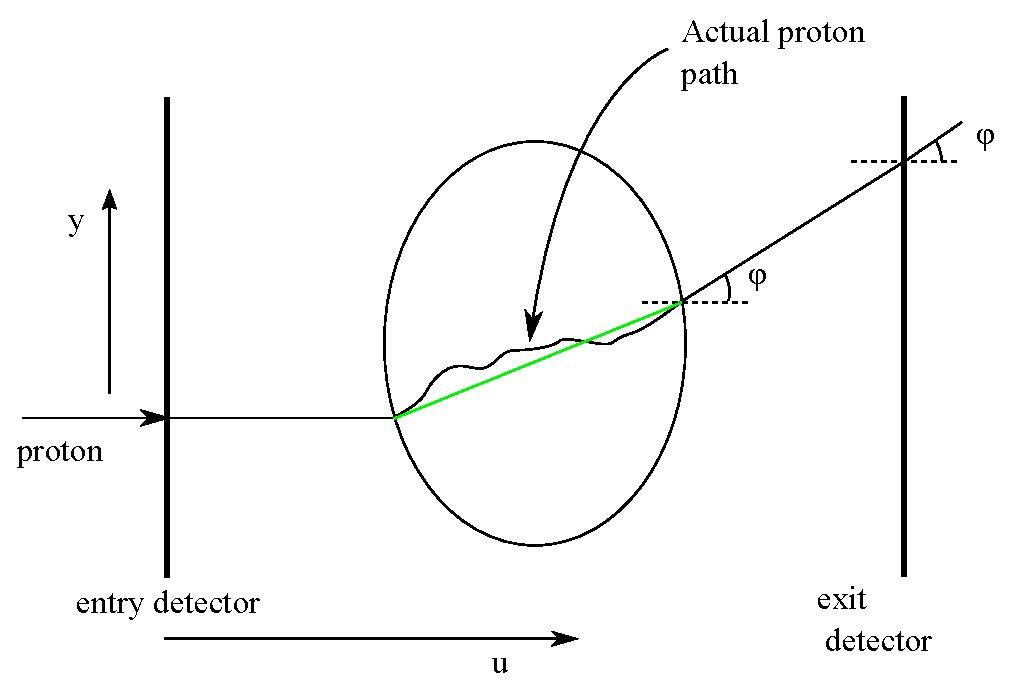
\includegraphics[scale=0.5]{img/mostlikelypath.eps}
\caption{(Exaggerated) track of a proton as it travels between two pCT detectors and through the elliptical phantom. In air (outside phantom) the path can be assumed to be straight and with negligible energy loss. In the phantom, the actual proton path follows a curved trajectory due to MCS. This path can be estimated as a straight path, cubic spline path or through the most likely path formalism (see appendix \ref{pathformalism}). The green line shows a straight path estimation for the proton.}
\label{fig:mlpphantom}
\end{figure}

\subsubsection{Filtering}
To reconstruct an image from the backprojection matrix, a filtering operation must be performed. It has been shown that the backprojection function, $b(x,y)$, is related to the original function being imaged, $f(x,y)$, by a 2D convolution (denoted by **) \cite{zeng1994backprojection}
\begin{eqnarray}
b(x,y) = f(x,y) ** \frac{1}{r}
\end{eqnarray}
where $r = |(x,y)|$. Due to the nature of the convolution, it is evident that outside the domain of the reconstruction region, where $f(x,y) = 0$, the backprojection $b(x,y)$ is non zero everywhere. Using the convolution theorem, it can be shown that the original image $f(x,y)$ can be obtained by 2D convolution with a spatial kernel $k(x,y)$,
\begin{align}
f(x,y) & = \mathcal{F}^{-1}\left(\frac{\mathcal{F}(b)}{\mathcal{F}(r^{-1})}\right) \\
& = b(x,y) ** \mathcal{F}^{-1}(\omega) \\
& = b(x,y) ** k(x,y)
\end{align}
where $\omega = |(\omega_x,\omega_y)|$ and $(\omega_x,\omega_y)$ are the conjugate frequency variables to $(x,y)$. The property that $\mathcal{F}(1/r) = \omega^{-1}$ has also been used. The kernel $k(x,y)$ can be obtained through a 2D inverse fourier transform of $\omega$. In computer implementation of the BPF algorithm, the backprojection region is discretised and is sampled at a frequency $1/\tau$. This frequency limit must also be imposed on the calculation of the spatial kernel. Poludniowski et al \cite{poludniowski2014proton} has shown the analytical form of $k(r)$ to be
\begin{align}
k(r) & = \mathcal{F}^{-1}(\omega) \\
& = \frac{1}{4\pi^2r^3}\left[\left(\frac{\pi r}{\tau}\right)^2 J_1\left(\frac{\pi r}{\tau}\right) - \phi\left(\frac{\pi r}{\tau}\right)\right] \\
\text{where} & \\
\phi(x) & = \frac{\pi x}{2} [ J_1(x) H_0(x) - J_0(x) H_1(x)]
\end{align}
where $J_n$ and $H_{n}$ are the $n^{th}$ order Bessel and Struve functions respectively. To avoid divergence and keep the kernel finite at $r = 0$, 
\begin{align}
k(r=0) = \frac{\pi}{12\tau^3}.
\end{align}
The imaged function in its discretised form is thus given by
\begin{eqnarray}
f[i,j] = b[i,j] ** k[i,j] 
\label{eq:bpconv}
\end{eqnarray}
where $f[i,j]$ is the discretised reconstruction matrix of size $N \times N$ and $i$ and $j$ are integer values, $i = 1 \dots N$  and $j = 1 \dots N$.

As in the FBP algorithm, the filtering operation is performed in the frequency domain after zero padding, and the original image can be obtained by
\begin{align}
f(x,y) = \tau^2 \times \mathcal{F}^{-1}\{\mathcal{F}(b(x,y) \text{ with zero padding}) \times \mathcal{F}(k(x,y) \text{ with zero padding})\} 
\end{align}

One of the problems that the BPF algorithm suffers from is a constant offset in the reconstructed values due to the need to truncate the backprojection matrix in equation \ref{eq:bpconv} \cite{suzuki1988comparison}. Poludniowski suggested a correction term, 

\begin{eqnarray}
\Delta = \left( \tau^2 \sum_{\substack{\text{pixels in}\\\text{reconstruction}\\\text{region}}} f[i,j] \right) \left( \tau^2 \sum_{\substack{\text{pixels not in}\\\text{reconstruction}\\\text{region}}} \frac{k[N/2 - i, N/2 - j]}{\tau\sqrt{i^2 + j^2}}\right)
\label{eq:correction}
\end{eqnarray}
that can be added onto the reconstructed values to achieve a quantitatively more accurate reconstruction.

\subsection{GEANT4}
\label{sec:geant4}
The GEANT4 (GEometry ANd	Tracking) simulation toolkit is a Monte Carlo based computer library written in C++ used to simulate particles propagating through and interacting with matter \cite{agostinelli2003geant4}. Initially developed for high energy particle physics applications, the software is now commonly used in medical applications. Using GEANT4, protons can be generated and tracked as they travel through a phantom medium, detectors can be designed to measure quantities such as energy and dose, and the results of the simulation can be visualised. Furthermore, an abundance of physical processes are available to handle the diverse interactions that may occur over a wide energy range. The user must select an appropriate physics model for the simulation being run. The validity of the physics model can be benchmarked by comparing to experimental results. Simulations that were performed in this project will be using GEANT4 10.2. RSP reconstructions and analysis of the results were performed in MATLAB 2014a.

\subsection{Spatial resolution and accuracy}
The quality of the image obtained through pCT can be assessed through measurements of the spatial resolution and the accuracy of the relative stopping power. There are various ways in which spatial resolution can be measured. For the purposes of this project, the modulation transfer function (MTF) has been used.

The MTF is measured in the frequency domain and by definition provides the contrast of a given spatial frequency relative to lower frequencies. Higher spatial frequencies in an image correspond to finer image detail, and increasing image detail becomes increasingly difficult to resolve. Thus intuitively one would expect the MTF to decrease with increasing spatial frequency as the contrast decreases and finer details become less distinguishable in the image. 

The MTF can be computed from the line spread function (LSF), which is derived from the derivative of the edge response function (ERF),
\begin{align}
\text{LSF}(x) = \frac{d}{dx}\text{ERF}(x)
\end{align}
The ERF is a line profile across an edge in an image and describes how an imaging system responds to a sharp discontinuity, while the LSF describes how an imaging system responds to a line. The MTF is the fourier transform of the LSF,
\begin{align}
\text{MTF}(w) = \mathcal{F}(\text{LSF}(x))
\end{align}

The MTF is usually normalised such that MTF$(\omega=0) =1$. The spatial resolution is often stated as the spatial frequency at which the MTF drops to 3-5\% of its maximum value. For images containing noise, this is difficult to assess without smoothing of the LSF or of the image, which is equivalent to a low pass filter.

To further compare images obtained, a special phantom has been designed consisting of slits of varying width and spacing (see figure \ref{fig:phantomSlit}). Line profiles through the slit can be used to compare the spatial resolution between images.

Assessment of the accuracy of the relative stopping power obtained from the reconstructions can be performed by comparing the mean stopping power of a region of interest of a certain material in the reconstructed image to the known stopping power. The materials used in the phantoms were water, air and bone, with relative stopping powers of 1.0, 0.0011 and 1.7321 respectively. The materials used came from the NIST reference database \cite{nist}. The RSPs were obtained directly from GEANT4 using the TestEm0 example application packaged with the toolkit. The example was modified to print proton stopping powers for the reference physics list, QGSP\_BERT, used in this project, at energies of 200 MeV.

%\subsection{Imaging dose}
%To be decided...

%\subsection{Merit function}
%To be decided...

%\newpage
\subsection{Simulations}
The simulated proton CT data was obtained using GEANT4 10.2 \cite{agostinelli2003geant4} with the reference physics list provided with the toolkit, QGSP\_BERT, that governs the physical processes and interaction probabilities. This physics list was chosen as it includes standard electromagnetic and hadronic processes. RSP reconstruction from the simulated data was performed using MATLAB 2014a. Calculation of the Struve functions for the filtering step in the BPF algorithm was performed used the FOTRAN library routines by Zhang and Jin \cite{zhang16computation} translated into MATLAB code using the MATLAB community developed software, f2matlab \cite{f2matlab}.

Two elliptical phantoms, of height 10 cm and major and minor axis of 16 cm and 14 cm respectively, were designed in a similar manner to \cite{li2006reconstruction}. The dimensions of the phantom were selected as such due to the expectation of a high percentage of pediatric patients being treated with protons. The phantoms consist of a cylindrical 1 cm shell of bone material (GEANT4: G4\_BONE\_COMPACT\_ICRU) in an environment containing air (GEANT4: G4\_AIR). Enclosed within the shell is water (GEANT: G4\_WATER). Within the shell of the first phantom, referred to as the slit phantom, 1 cm $\times$ 1 cm squares are placed consisting of a varying number of lines of either bone or air (1 - 5 lp/cm (line pairs per cm)). The second phantom, which is referred to as the edge phantom, is identical to the slit phantom but with the slits replaced by two $4 \times 5 \times 10$ cm rectangular blocks of air and bone. The phantoms are shown in figure \ref{fig:phantomSlit}.

\begin{figure}[htp]
  % Fixed length
  \centering
  \subcaptionbox{\label{fig3:a}}{\includegraphics[width=0.295\linewidth]{img/geant4.png}}\hspace{0.5em}%
 \subcaptionbox{\label{fig3:b}}{\includegraphics[width=0.3\linewidth]{img/slitPhantom.png}}
 \subcaptionbox{\label{fig3:b}}{\includegraphics[width=0.3\linewidth]{img/edgePhantom.png}}
 \caption{GEANT4 elliptical phantom containing air and bone, surrounded by an elliptical shell of bone. The red squares are the detectors.}
\label{fig:phantomSlit}
\end{figure}

Detectors were placed before and after the phantom, 23 cm away from the isocentre, that recorded the position, direction and kinetic energy of each proton, and protons were tracked individually. A uniformly distributed proton beam of 200 MeV with no energy distribution and divergence was used. The choice of energy was chosen as the Bragg peak will be located outside of the phantom as well as being an attainable energy in a clinical setting. The beam spanned a 23 cm line parallel to the detector, with the proton direction perpendicular to the detectors and towards the phantom. Higher energies can be used, but in proton therapy centres there will be an upper limit on proton energies, governed by the apparatus. Protons were fired from immediately behind the first detector. $10^5$ protons were generated in $1^{\circ}$ intervals between $0^{\circ}$ and $179^{\circ}$.

A crude estimation of the dose deposited in the phantom was carried out by considering the change in energies between the first and last detector. The slit and edge phantom resulted in changes in proton energy of $6.4 \times 10^8$ MeV and $6.3 \times 10^8$ MeV respectively. The dose deposited per unit volume was then computed by assuming the volume imaged to be of height, $h = 1$ mm so that the volume $V = \pi a b h$, where $a$ and $b$ are the radii of the elliptical phantom. The imaging dose was then found to be 4.8 mGy.

%\newpage
\section{Results}
\subsection{Filtered backprojection}
\label{sec:results}
The FBP method was used to reconstruct a map of the RSP inside the slit phantoms. Protons that did not reach the second detector were not used for the reconstruction (0.01\% of initial protons). As the FBP method assumes straight imaging particle paths, protons that had deviated from their original lateral position by more than 1 mm were removed from the reconstruction. This can be performed in practice using the tracking detectors discussed in section \ref{sec:detector}. The lateral position of the incident proton beam was binned in 1 mm bins and the path of the protons was assumed to be straight and was binned according to the detected position of the protons at the first detector. The reconstructed images of relative stopping power with and without the removal of protons deviating more than 1 mm from the reconstruction are shown in figure \ref{fig:fbpPhantomSlitImage}.


\begin{figure}[!htpb]
  % Fixed length
  \centering
  \subcaptionbox{\label{fig3:a}}{\includegraphics[width=0.3\linewidth]{img/fbpUnfiltered.jpg}}\hspace{2em}%
 \subcaptionbox{\label{fig3:b}}{\includegraphics[width=0.3\linewidth]{img/fbpFiltered.jpg}} \\
%  \subcaptionbox{\label{fig3:a}}{\includegraphics[width=0.4\linewidth]{img/FBPRSPUnfiltered.jpg}}\hspace{2em}%
% \subcaptionbox{\label{fig3:b}}{\includegraphics[width=0.4\linewidth]{img/FBPRSPFiltered.jpg}} \\ 
  \subcaptionbox{\label{fig3:a}}{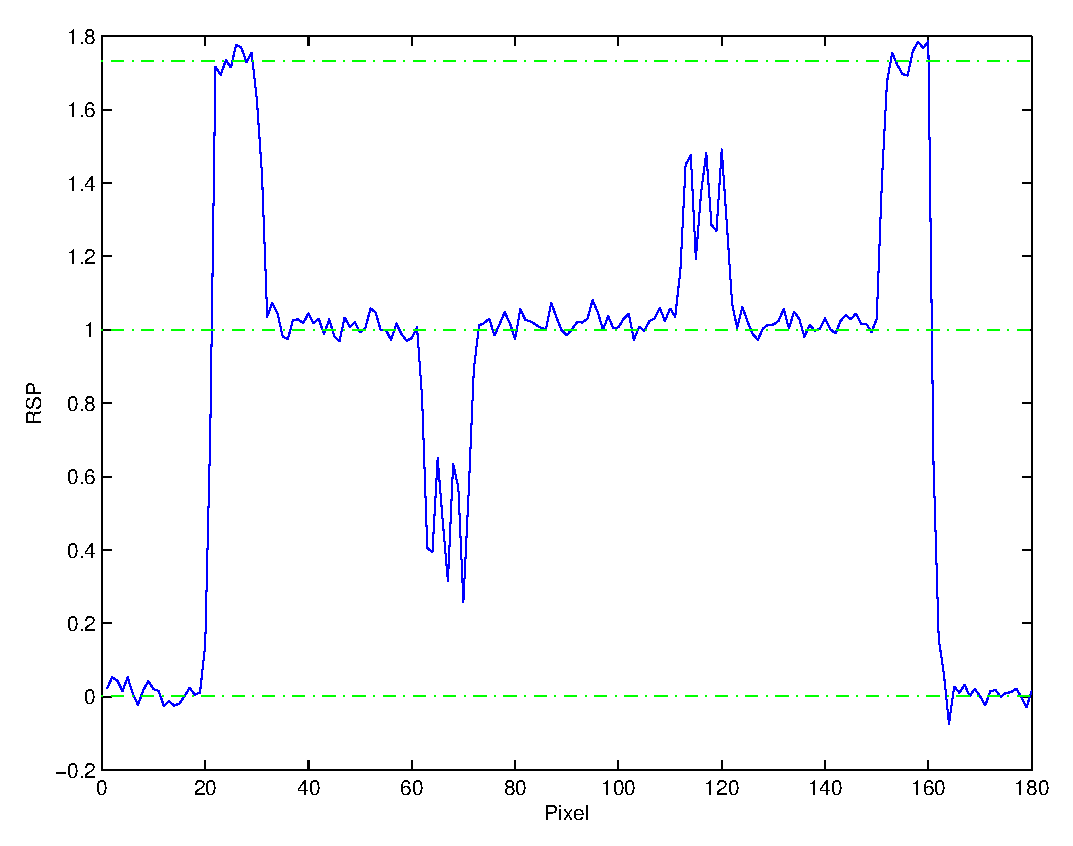
\includegraphics[width=0.4\linewidth]{img/fbpCentreUnfilt.eps}}\hspace{2em}%
 \subcaptionbox{\label{fig3:b}}{\includegraphics[width=0.4\linewidth]{img/fbpCentreFilt.eps}} \\ 
   \subcaptionbox{\label{fig3:a}}{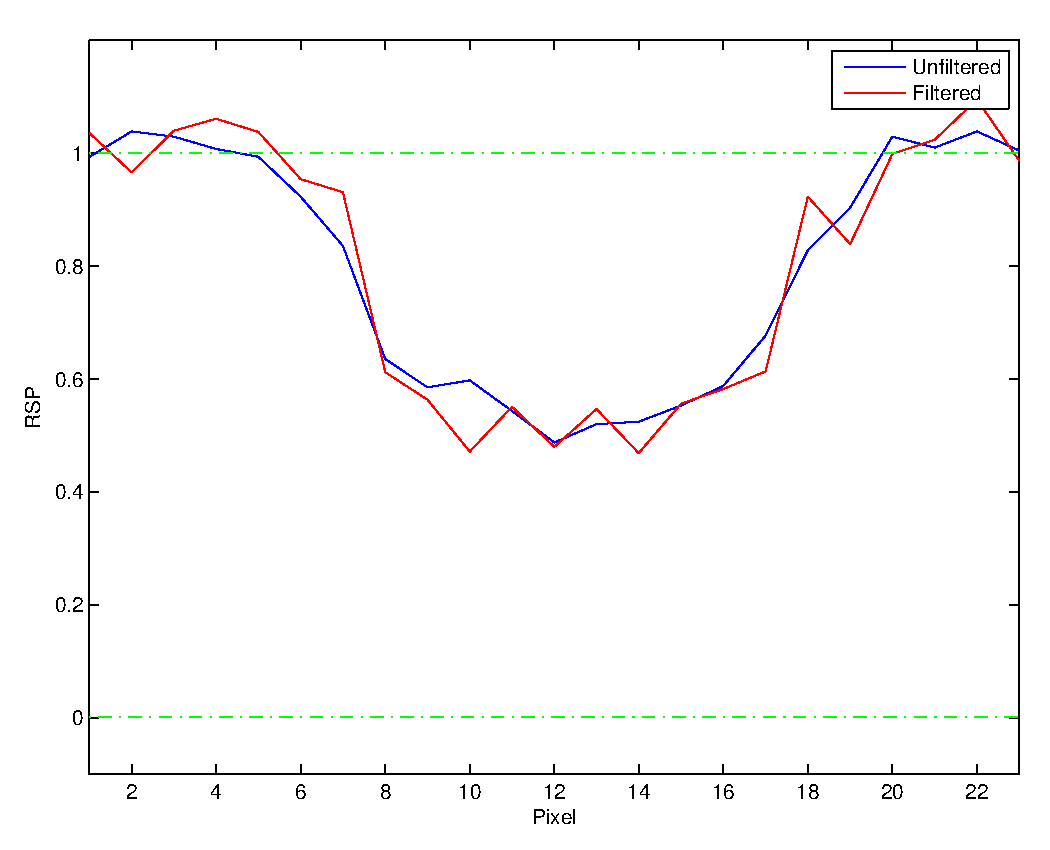
\includegraphics[width=0.4\linewidth]{img/fbpSlitAir.eps}}\hspace{2em}%
 \subcaptionbox{\label{fig3:b}}{\includegraphics[width=0.4\linewidth]{img/fbpSlitBone.eps}} \\ 
\caption{Reconstructed 2D slice of phantom using FBP. (a): using all protons detected at the detector after the reconstruction region. (b): protons that had a lateral displacement more than 1 mm from their original position were omitted from the reconstruction. (c),(d): the blue line is the relative stopping power of a line through centre of phantom, the green-dashed line is relative stopping powers of water (1.00), air (0.0011) and bone (1.7321). (e): line profiles through centre of 5 lp/cm slits of air, (f): line profiles through centre of 5 lp/cm slits of bone.}
\label{fig:fbpPhantomSlitImage}
\end{figure}

It is immediately evident from figure \ref{fig:fbpPhantomSlitImage} that the spatial resolution of the image is improved after removal of protons that had deviated from their original position by more than 1 mm. The fraction of protons used in the reconstruction after filtering the proton data ranged between 0.49 and 0.56 (see figure \ref{fig:fbpFracFilt}).

\begin{figure}[!htpb]
\centering
\includegraphics[scale=0.5]{img/fbpFracFilt.jpg}
\caption{The fraction of protons used in the FBP reconstruction as a function of view angle. The criteria for removal was a difference of more than 1 mm between detected lateral positions at the first and second detector.}
\label{fig:fbpFracFilt}
\end{figure}

\FloatBarrier


\subsection{Most likely path in water}
Implementation of the MLP for protons travelling through 20 cm of water using GEANT4 was performed as per \cite{schulte2008maximum}. Only the lateral position was considered as the perpendicular deflection directions can be taken independently. As required for the MLP calculation, $1/(\beta^2 p^2)$ was fitted to a $5^{th}$ degree polynomial, $1/(\beta^2 p^2) = \sum_{i=0}^5 a_{i} u^i$, where $u$ is the depth of penetration of the proton, $\beta$ is the speed of the proton relative to the speed of light, and $p$ is the momentum of the proton. The polynomial coefficients computed are shown in table \ref{coefficients}, and vary slightly from the literature \cite{schulte2008maximum,williams2004most}. This is likely due to the choice of physics model used in the GEANT4 simulation (physics list used: QGSP\textunderscore BERT). Some proton trajectories along with their predicted MLP are shown in figure \ref{fig:mlp}. 
%\vspace{1cm}

\begin{table}[h]
\centering
\caption{Polynomial coefficients used to the fit the curve $1/(\beta^2 p^2) = \sum_{i=0}^5 a_i u^i$. The coefficients $a_{i}$ are in units of c$^2$/MeV divided by appropriate powers of cm. Strict cuts of $3\sigma$ were applied on proton kinetic energy and on exit angle relative to entry angle before fitting.}
\begin{tabular}{l|c}
\hline
Coefficient & $a_{i}$ (c$^2$/(MeV cm$^{i})$) \\ \hline
$a_0$ & $7.4361\times 10^{-6}$ \\
$a_1$ & $5.0199\times 10^{-7}$ \\
$a_2$ & $-7.8071 \times 10^{-8}$ \\ 
$a_3$ & $1.5860 \times 10^{-8}$ \\
$a_4$ & $-1.0912 \times 10^{-9}$ \\
$a_5$ & $3.0185 \times 10^{-11}$  \\
\end{tabular} 

\label{coefficients}
\end{table}

\begin{figure}[!htb]
  \hspace*{\fill}%
  \subcaptionbox{}{\includegraphics[width=2.5in]{img/MLP1.jpg}}\hfill%
  \subcaptionbox{}{\includegraphics[width=2.5in]{img/MLP2.jpg}}%\hfill
  \hspace*{\fill}\\
  
  \hspace*{\fill}%
  \subcaptionbox{}{\includegraphics[width=2.5in]{img/MLP3.jpg}}\hfill%
  \subcaptionbox{}{\includegraphics[width=2.5in]{img/MLP4.jpg}}%\hfill
  \hspace*{\fill}
  \caption{The most likely path (MLP) formalism implemented for protons travelling through a water medium of 20 cm depth. The solid red line is the simulated proton path in water, measured every 0.5 cm. The solid blue line is the MLP of the proton calculated using the ingoing and outgoing positions and angles (at a depth of 0 cm and 20 cm respectively). The dashed blue line is the 1$\sigma$ envelope predicted by the MLP formalism. The lower two figures show the rare cases when the proton travels outside the $1\sigma$ envelope.}
\label{fig:mlp}
\end{figure}

%\begin{figure}[!h]
%%\centering
%\makebox[\linewidth][c]{
%\begin{subfigure}[b]{.6\linewidth}
%  \centering
%  \includegraphics[width=0.9\textwidth]{img/MLP1.jpg}
%  \caption{ }
%  \label{fig:sub1}
%\end{subfigure}
%\begin{subfigure}[b]{.6\linewidth}
%  \centering
%  \includegraphics[width=0.9\textwidth]{img/MLP2.jpg}
%  \caption{ }
%  \label{fig:sub2}
%\end{subfigure}} \\
%\makebox[\linewidth][c]{
%\begin{subfigure}[b]{.6\linewidth}
%  \centering
%  \includegraphics[width=0.9\textwidth]{img/MLP3.jpg}
%  \caption{ }
%  \label{fig:sub2}
%\end{subfigure}
%\begin{subfigure}[b]{.6\linewidth}
%  \centering
%  \includegraphics[width=0.9\textwidth]{img/MLP4.jpg}
%  \caption{ }
%  \label{fig:sub2}
%\end{subfigure}}
%\caption{The most likely path (MLP) formalism implemented for protons travelling through a water medium of 20 cm depth. The solid red line is the simulated proton path in water, measured every 0.5 cm. The solid blue line is the MLP of the proton calculated using the ingoing and outgoing positions and angles (at a depth of 0 cm and 20 cm respectively). The dashed blue line is the 1$\sigma$ envelope predicted by the MLP formalism. The lower two figures show the rare cases when the proton travels outside the $1\sigma$ envelope.}
%\label{fig:mlp}
%\end{figure}

\subsection{Most likely path in phantom}
The most likely path formalism was used to predict the path of the protons within the phantoms. The exact paths of 5000 protons were recorded between the two detectors and passing through the centre of the slit phantom. The actual paths of the protons were compared to that predicted by the most likely path, a straight path and a cubic spline path, and the root mean square error is shown in figure \ref{fig:mlpInPhantom}. In the path estimation it was assumed that there was no energy loss or straggling between the detectors and the phantom, which in reality is minimal in air, and thus the entry and exit angle at the phantom boundaries were equal to those measured at the detector. Between the phantom and detectors it was assumed the protons travelled in straight lines (see figure \ref{fig:mlpphantom}). Both the cubic spline and MLP estimations show a significant improvement and lower RMS errors than a straight path estimation, however the difference between the cubic spline and MLP does not appear to be significantly different.

\begin{figure}[!htb]
  \hspace*{\fill}%
  \subcaptionbox{$0^{\circ}$ rotated phantom}{\includegraphics[width=3.0in]{img/rms0.eps}}\hfill%
  \subcaptionbox{$90^{\circ}$ rotated phantom}{\includegraphics[width=3.0in]{img/rms90.eps}}%
  \hspace*{\fill}\\
  \caption{Plots of the RMS error of the predicted paths of protons using the straight line method and the most likely path. (a) is when the phantom is oriented as in figure \ref{fig:mlpphantom} and (b) is when the phantom has been rotated by $90^{\circ}$.}
\label{fig:mlpInPhantom}
  \end{figure}

%\begin{figure}[!h]
%%\centering
%\makebox[\linewidth][c]{
%\begin{subfigure}[b]{.6\linewidth}
%  \centering
%  \includegraphics[width=0.8\textwidth]{img/rms0.eps}
%  \caption{$0^{\circ}$ rotated phantom}
%  \label{fig:sub1}
%\end{subfigure}%
%\begin{subfigure}[b]{.6\linewidth}
%  \centering
%  \includegraphics[width=0.8\textwidth]{img/rms90.eps}
%  \caption{$90^{\circ}$ rotated phantom}
%  \label{fig:sub2}
%\end{subfigure}
%}
%\caption{Plots of the RMS error of the predicted paths of protons using the straight line method and the most likely path. (a) is when the phantom is oriented as in figure \ref{fig:mlpphantom} and (b) is when the phantom has been rotated by $90^{\circ}$.}
%\label{fig:mlpInPhantom}
%\end{figure}

\FloatBarrier

\subsection{Backprojection-then-filtering}
RSP reconstructions of the two phantoms were performed using the BPF algorithm. The reconstruction and backprojection areas were discretised into 1 mm $\times $ 1 mm and 0.5 mm $\times$ 0.5 mm voxels for the edge phantom, and 0.5 mm $\times$ 0.5 mm voxels for the slit phantom. The larger voxel size was chosen to assess RSP accuracy while the finer reconstruction region was to assess spatial resolution. The three different proton path estimates were used. $3 \sigma$ cuts on relative exit angle and on lateral position were imposed on the data to filter out protons that had likely undergone an inelastic nuclear interaction (see section \ref{app:protoninteractions}). Unless otherwise stated, the images were Gaussian blurred by convolving them with a $3 \times 3$ Gaussian filter with $\sigma = 1/\sqrt{2}$ to reduce the noise. The reconstructed images are shown in figure \ref{fig:bpfRSP}. An immediate improvement in spatial resolution compared to the FBP method can be observed. The cubic spline path and most likely path estimations do not appear to differ significantly in spatial resolution, however both show an improvement in comparison to the straight path estimate. 

Three regions of interest (ROI) were selected in the edge and slit phantom, and the mean value of the RSP within the area was computed without applying the correction term $\Delta$ to the reconstructed values (see tables \ref{table:edgeVals} and \ref{table:slitVals}). The three different path estimations did not appear to significantly affect the the reconstructed values. The mean value of the RSP for air was found to be negative. This would imply that the protons gain energy as they pass through air, which is obviously not the case. The miscalculation is likely to be a result of the very low stopping power in air and the noise in the image.

The correction term, $\Delta$, was not included in the RSP calculation because it ranged in values between -0.5 and -1.5.

\begin{figure}[!htb]
  \hspace*{\fill}%
  \subcaptionbox{}{\includegraphics[width=1.6in]{img/bpfEdgeLine.jpg}}\hfill%
  \subcaptionbox{}{\includegraphics[width=1.6in]{img/bpfEdgeSpline.jpg}}\hfill
  \subcaptionbox{}{\includegraphics[width=1.6in]{img/bpfEdgeMLP.jpg}}%
  \hspace*{\fill}\\
  
  \hspace*{\fill}%
  \subcaptionbox{}{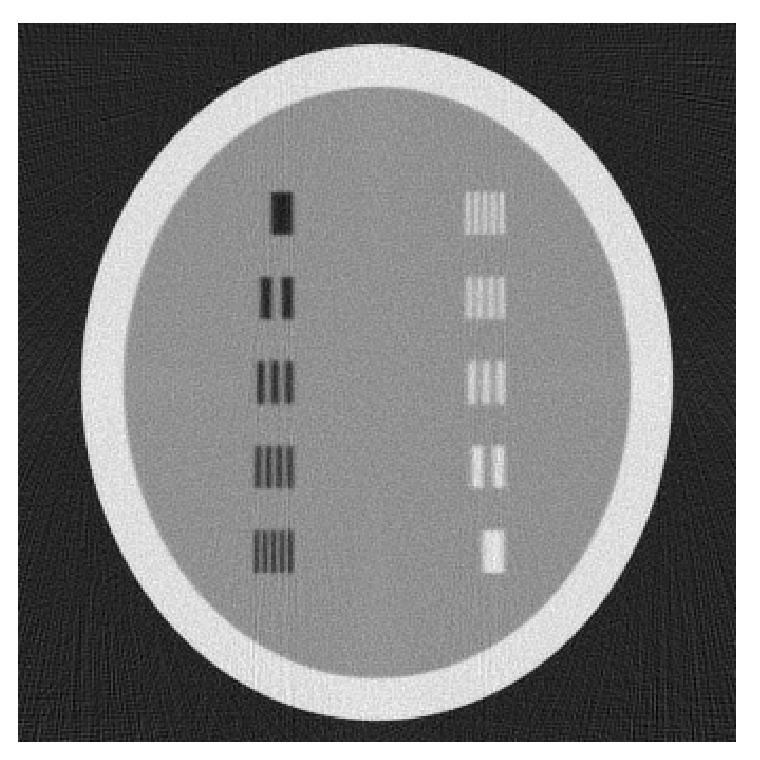
\includegraphics[width=1.653in]{img/slitFineLine.eps}}\hfill%
  \subcaptionbox{}{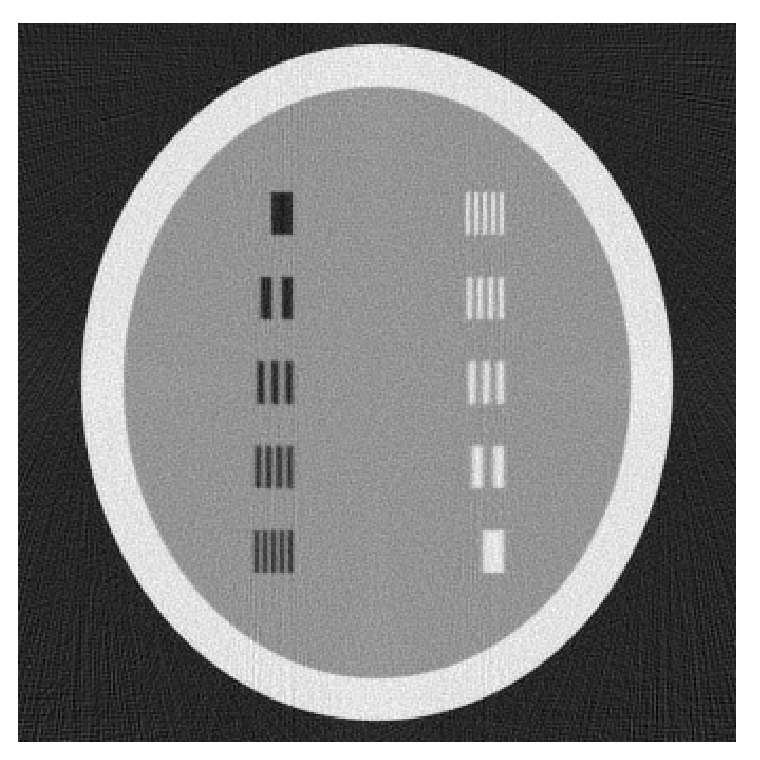
\includegraphics[width=1.653in]{img/slitFineSpline.eps}}\hfill
%  \subcaptionbox{}{\includegraphics[width=1.6in]{img/bpfSlitMLP.jpg}}%
  \subcaptionbox{}{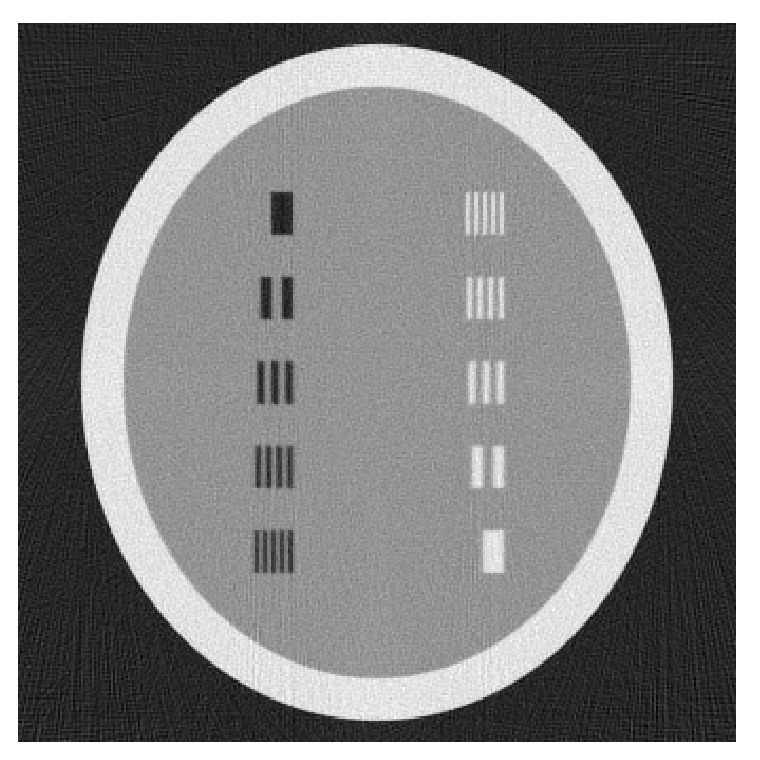
\includegraphics[width=1.653in]{img/slitFine.eps}}  
  \hspace*{\fill}
  \caption{Reconstructed RSP maps using the BPF algorithm. From left to right: straight path, cubic spline, most likely path estimation. Images reconstructed on a $0.5 \times 0.5$ mm$^2$ voxel grid.}
  \label{fig:bpfRSP}
\end{figure}

%%%%%%%%%%% this table is with 0.5 mm x 0.5 mm
%\begin{table}[!htb]
%\centering
%\caption{Mean reconstructed RSP values in three regions of interest in the edge phantom. The ROIs contain either air, water or bone. The standard deviation was used to assess the noise in each ROI.}
%\begin{tabular}{l|cccc}
%\hline
%Material & RSP & Standard deviation, $\sigma$ \\ \hline
%Air (Straight line) & 0.0012 & 0.0287 & \\
%Air (Spline) & 0.0016 & 0.0306 & \\
%Air (MLP) & 0.0016 & 0.0303 & \\
%Water (Straight line) & 1.0116 & 0.0339  \\
%Water (Spline) & 1.0116 & 0.0339  \\
%Water (MLP) & 1.0116 & 0.0341  \\
%Bone (Straight line) & 1.7573 & 0.0370 \\ 
%Bone (Spline) & 1.7578 & 0.0342 \\ 
%Bone (MLP) & 1.7578 & 0.0345 \\ 
%\end{tabular} 
%
%\label{table:edgeVals}
%\end{table}

\begin{table}[!htb]
\centering
\caption{Mean reconstructed RSP values in three regions of interest in the edge phantom (discretisation: $1 \times 1$ mm$^2$). The ROIs contain either air, water or bone. The standard deviation was used to assess the noise in each ROI.}
\begin{tabular}{l|cccc}
\hline
Material & RSP & Standard deviation, $\sigma$ & Percentage error\\ \hline
Air (Straight line) & -0.009705 & 0.005168 & 982\% \\
Air (Spline) & -0.009334 & 0.005202 & 949\%\\
Air (MLP) & -0.009293 & 0.005201 &  945\% \\
Water (Straight line) & 1.002056 & 0.007443 & 0.8\% \\
Water (Spline) & 1.001817 & 0.006157 & 0.2\% \\ 
Water (MLP) & 1.001801 & 0.006066  & 0.2\%\\
Bone (Straight line) & 1.745939 & 0.006022 & 0.8\%\\ 
Bone (Spline) & 1.746242 & 0.005899 & 0.8\%\\ 
Bone (MLP) & 1.746289 & 0.005790 & 0.8\%\\ 
\end{tabular} 

\label{table:edgeVals}
\end{table}


% slit phantom with 1 mm x 1mm voxels
\begin{table}[!htb]
\centering
\caption{Mean reconstructed RSP values in three regions of interest in the slit phantom (discretisation: $1 \times 1$ mm$^2$). The ROIs contain either air, water or bone. The standard deviation was used to assess the noise in each ROI.}
\begin{tabular}{l|cccc}
\hline
Material & RSP & Standard deviation, $\sigma$ & Percentage Error  \\ \hline
Air (Straight line) & 0.011007 & 0.030176 & 901\% \\
Air (Spline) & -0.000784 & 0.025603 & 171\%\\
Air (MLP) & -0.001424  & 0.024789 & 229\%\\

Water (Straight line) & 1.003654 & 0.008643 & 0.4\%\\
Water (Spline) & 1.003677 & 0.008569 & 0.4\%\\
Water (MLP) & 1.003685 & 0.008425 & 0.4\%\\

Bone (Straight line) & 1709807 & 0.021598 & 1.3\% \\ 
Bone (Spline) & 1.717965 & 0.017142 & 0.8\%\\ 
Bone (MLP) & 1.718519 & 0.016502 & 0.8\%\\ 
\end{tabular} 
\label{table:slitVals}
\end{table}


%%% with 0.5 mm x 0.5 mm voxels!
%\begin{table}[!htb]
%\centering
%\begin{tabular}{l|cccc}
%\hline
%Material & RSP & Standard deviation, $\sigma$  \\ \hline
%Air (Straight line) & 0.001890 & 0.076572 \\
%Air (Spline) & 0.003849 & 0.072135 \\
%Air (MLP) & 0.002644  & 0.075357 \\
%
%Water (Straight line) & 1.015259 & 0.061875 \\
%Water (Spline) & 1.015312 & 0.060458 \\
%Water (MLP) & 1.015348 & 0.060099 \\
%
%Bone (Straight line) & 1.725730 & 0.090227 \\ 
%Bone (Spline) & 1.741086 & 0.067993 \\ 
%Bone (MLP) & 1.741676 & 0.068392 \\ 
%\end{tabular} 
%\caption{Mean reconstructed RSP values in three regions of interest in the slit phantom. The ROIs contain either air, water or bone. The standard deviation was used to assess the noise in each ROI.}
%\label{table:slitVals}
%\end{table}

Line profiles through the slits in the slit phantom were further used to assess the spatial resolution (see figure \ref{fig:bpfLineProfile}). The line profiles show more distinct peaks and troughs using the cubic spline path and MLP estimations than the straight line path, yet there was no significant difference between cubic spline and MLP estimations.

\begin{figure}[!htb]
  \hspace*{\fill}%
  \subcaptionbox{}{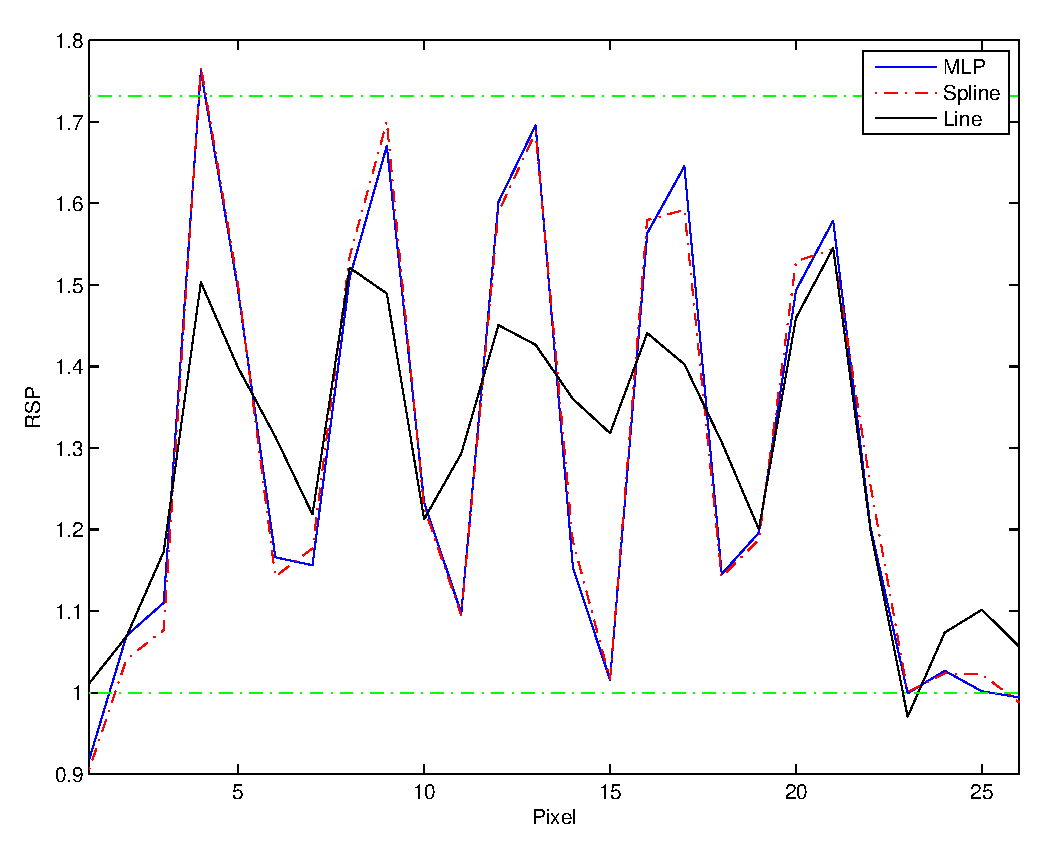
\includegraphics[width=2.5in]{img/graphSlit1New.eps}}\hfill%
  \subcaptionbox{}{\includegraphics[width=2.5in]{img/graphSlit2New.eps}}%
  \hspace*{\fill}\\
%  \hspace*{\fill}
%  \subcaptionbox{}{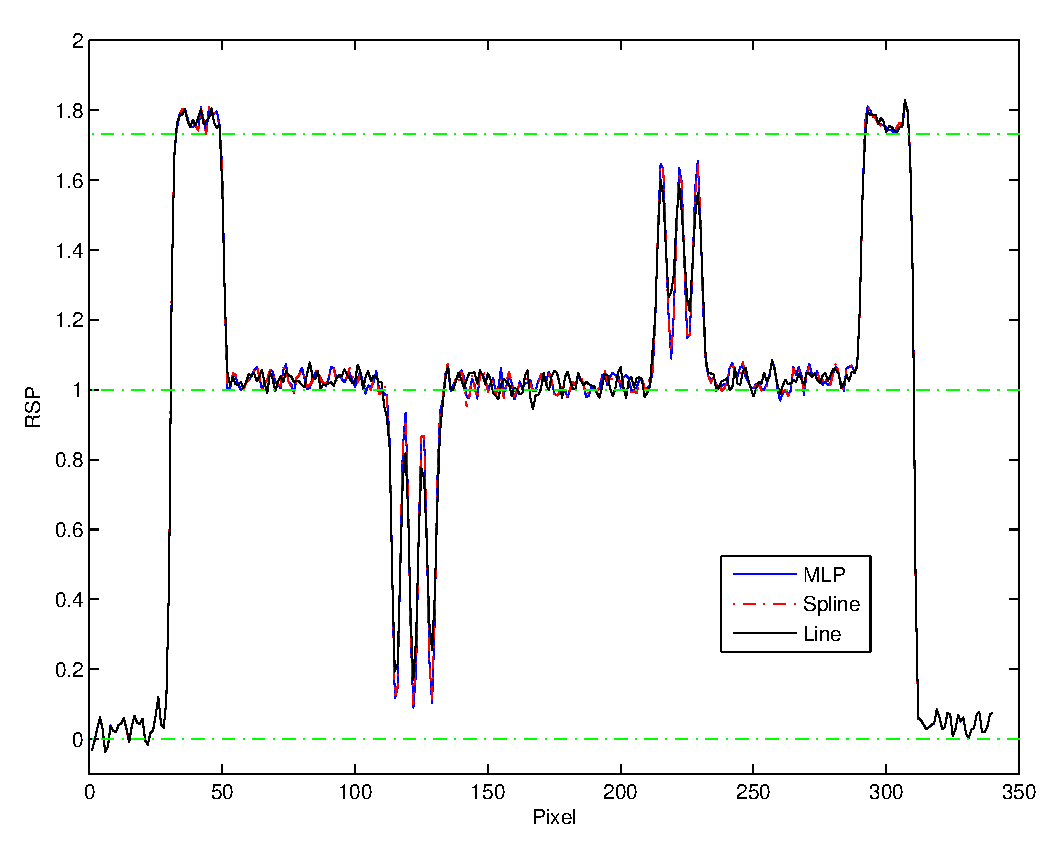
\includegraphics[width=4in]{img/graphSlit3.eps}}%
%  \hspace*{\fill}\\
  \caption{Line profile through (a) slits containing bone (5 lp/cm), (b) slits containing air (5 lp/cm). (discretisation: $0.5 \times 0.5$ mm$^2$, no Gaussian blurring)}% (c) horizontal slice through centre of phantom.}
  \label{fig:bpfLineProfile}
\end{figure}

The modulation transfer function was used to assess the difference in spatial resolution given by the different path estimations. The normalised MTF was found from the boundaries between water and air and water and bone in the edge phantom, and can be seen in figure \ref{fig:bpfMTF}. 80 line profiles from each vertical edge were taken across each vertical boundary and averaged to minimise noise artefacts (mean line profile averaged over 160 line profiles from both vertical edges for each square). It can be seen that for frequencies below $\sim 0.5$ cycles/mm, the MLP and cubic spline path estimations result in MTF curves that fall more steadily than that of the straight path estimate. There is a slight improvement in MTF using the MLP when compared to the cubic spline. 

\begin{figure}[!htb]
  \hspace*{\fill}%
  \subcaptionbox{}{\includegraphics[width=2.5in]{img/MTFsmoothingAir.eps}}\hfill%
  \subcaptionbox{}{\includegraphics[width=2.5in]{img/MTFsmoothingBone.eps}}%
  \hspace*{\fill}\\
  \caption{Normalised MTF function: (a) boundary used was between water and air, (b) boundary used was between water and bone. (discretisation: $0.5 \times 0.5$ mm$^2$)}
  \label{fig:bpfMTF}
\end{figure}



%\FloatBarrier
%\newpage
%\subsection{Spatial resolution \& RSP accuracy}
%A phantom was specifically designed to consist of edges to determine the spatial resolution of reconstructions (see figure (fig)). The phantom is identical to the elliptical phantom as before with the slits replaced by two rectangular (5 x 4 x 10 cm) volumes, one composed of air and the other of bone. The reconstructed image using FBP and BPF are shown in figure.

%\begin{figure}[!ht]
%%\centering
%\makebox[\linewidth][c]{
%\begin{subfigure}[b]{.5\linewidth}
%  \centering
%  \includegraphics[width=0.9\textwidth]{img/fbpEdge.jpg}
%  \caption{Using FBP}
%  \label{fig:sub1}
%\end{subfigure}%
%\begin{subfigure}[b]{.5\linewidth}
%  \centering
%  \includegraphics[width=.9\textwidth]{img/bpfEdge.jpg}
%  \caption{Using BPF}
%  \label{fig:sub2}
%\end{subfigure}
%} \\
%\makebox[1.0\linewidth][c]{
%\begin{subfigure}[b]{1.1\linewidth}
%  \includegraphics[width=1.0\linewidth]{img/EdgeLineProfile.jpg}
%\end{subfigure}
%}
%\end{figure}

%\subsection{Parallel beam reconstruction}
%\subsection{Fan beam reconstruction}
%If I successfully manage to implement!

\section{Discussion}
The RSP reconstructions produced using the FBP method exhibited a lower spatial resolution than those when using the BPF algorithm, even after filtering protons that deviated more than 1 mm from their initial position as measured at the entry detector. This is in large part due to the fact that approximately 50\% of the protons had to be omitted from the reconstruction as they excessively deviated from a straight path trajectory. One could increase the number of protons used to image the phantom and this should increase the spatial resolution of the images produced using FBP. However, 50\% of the protons would still be unusable yet would contribute to the dose deposited to the phantom.

The BPF algorithm, on the other hand, produced RSP maps that were of a higher spatial resolution. The highest spatial resolution was observed when using the most likely path estimation. However, it did not appear to be a significant improvement on that produced using the cubic spline path. Both cubic spline and MLP estimations showed a significant improvement in spatial resolution when compared to a straight line path estimation.

The BPF algorithm without using the correction term overestimated the RSP in the regions of interest selected for both water and bone. This is likely due to the truncation of the backprojection matrix in equation \ref{eq:bpconv}. In reality, the backprojection matrix is infinitely big, and in a computer implementation needs to be truncated. In the implementation used for this project, the backprojection matrix covered an area of $23 \times 23$ cm$^2$. A larger backprojection matrix should result in more quantitatively accurate results with a computational cost in both memory and time for backprojection. The correction term proposed by Poludniowski et al \cite{poludniowski2014proton} (see equation \ref{eq:correction}) was intended to compensate for this truncation. However, it was not implemented in this project. Nevertheless, the RSPs reconstructed for both water and bone were well within the accuracy desired for pCT ($< 1$\%). On the other hand, all three path estimations underestimated the RSP of the ROI containing air, and produced mean negative values. This is possibly due to all three path estimations being considerably different to that traversed by the proton in that region of the phantom, and is a subject for further study.

The standard deviation, or equivalently noise, was lowest when using the most likely path estimation. Noise in the image when using the BPF algorithm is a subject of interest in future work as a thorough understanding of the propagation of noise from the algorithm and the parameters that affect will aid in producing an optimal signal.

The most time consuming step of the BPF algorithm is the backprojection of the proton paths. Siddon's algorithm \cite{siddon1985fast} was used to determine the pixels intersected and path length traversed through each pixel by individual protons. This can likely be sped up by using more modern algorithms \cite{jacobs1998fast}. For a $23 \times 23$ cm$^2$ backprojection region discretised into $1 \times 1$ mm$^2$ voxels, the backprojection of $10^5$ protons from 180 angles took approximately 5 hours on a quad core computer. It is important to note here that the backprojection step is highly parallelisable. With the use of GPUs, that can handle thousands of threads simultaneously, the time for the backprojection step can greatly be reduced. The filtering stage takes approximately 10 seconds on a typical home computer.

It should be noted that the set up used in GEANT4 was an idealised set up with perfect detectors to track the position, direction and energies of the individual protons, from which the proton paths were estimated. Similarly, the protons used had no spread in energies and the beam line was ideal. In reality, tracking will be limited by the resolution of the detectors used and proton beam energies will be spread. These factors can be implemented in GEANT4. Also, the usage of the QGSP\_BERT physics list used in the pCT simulations can be extended, customised and then benchmarked against real pCT data to allow for more accurate modelling.

Furthermore, this project limited the imaging to a plane using parallel beam CT. The BPF algorithm should naturally extend to fan and cone beam CT, and can be used to reconstruct a 3D volume through sequential planar imaging. 

Researchers have investigated other approaches to the backprojection-then-filtering method for computed tomography. Zeng et al proposed a BPF algorithm that alleviates the need for an unbounded backprojection region and hence avoiding inaccuracies due to truncation in the filtering stage \cite{zeng2007image}. In 2015, Rit et al applied this method to proton CT \cite{ritlist}.

A crude estimation of the dose deposited in the phantom was used in this project by taking the difference in detected energies before and after the phantom. This does not account for secondary particles that may deposit their energy outside of the phantom. Future work should involve a more accurate dose deposition, particularly when comparing proton CT to other imaging modalities in the determination of RSP.

\section{Conclusion}
The filtered backprojection and backprojection-then-filtering reconstruction algorithms have been applied to RSP reconstruction from data obtained using proton CT. Two elliptical shaped phantoms consisting of air, water and bone materials were imaged using protons. The proton CT data acquired through Monte Carlo simulations using the GEANT4 simulation toolkit. RSP accuracy for both bone and water materials matched the $< 1$\% accuracy desired of pCT, however, this was not achieved for air. The backprojection then filtering algorithm appears suitable for use in proton treatment planning. 

\section{Acknowledgements}
I would like to thank Dr Michael Merchant for his constant support and advice throughout this project. I would also like to thank the team working with GEANT4 at the University of Manchester for always allowing me to bounce ideas of them and sharing their knowledge in GEANT4 with me. Finally, thank you to professor Karen Kirkby and the PRECISE team (Proton Research at the Christie and Institute of Cancer Sciences) for welcoming me into the team at the University of Manchester.


\newpage
\appendix 
\section{Introduction}
\label{app:intro}
Until recently, the fraction of radiotherapy clinics utilising proton therapy has been small, largely due to the relatively high beam energies required and associated high costs - but this is increasing with advances in technology \cite{schulte2004conceptual}. Proton radiation therapy offers the distinct advantage over conventional forms of radiation therapy by providing the possibility of precisely irradiating the tumour volume while depositing only a low dose of radiation to healthy tissue. 

It was in 1946 that Robert Wilson first proposed the use of protons as an alternative form of therapeutic treatment due to their high ionisation per unit path traversed \cite{wilson1946radiological}. Their precise dose deposition is a consequence of the fact that the ionisation by a proton is proportional to the inverse square of its velocity. This results in protons exhibiting a peak dose, known as a Bragg peak, moments before they come to rest, and depositing a minimal dose in traversing a material up until the Bragg peak. The depth in a material at which the Bragg peak occurs can be varied by selecting an appropriate energy of the incident proton beam, and a spread out Bragg peak (SOBP) is formed to irradiate a tumour volume by using a range of proton energies (see figure \ref{fig:braggpeak}). These attributes of protons provide a significant benefit - they have the ability to produce a highly conformal dose distribution at the malignant tissue while minimising the dose to healthy tissue. This is in contrast to more conventional photon radiotherapy, which deposits a relatively high dose to healthy tissue and continues to traverse the body and deposit energy after passing the tumour.
\begin{figure}[h]
\centering
\includegraphics[scale=1]{img/braggpeak.jpg}
\caption{Depth-dose distribution for the spread out Bragg peak (SOBP) (red), its constituent Bragg peaks (blue) and for a 10 MV photon beam (black). Image adapted from \cite{levin2005proton}}
\label{fig:braggpeak}
\end{figure}

All radiotherapy treatment is preceded by treatment planning and verification of the tumour volume. Due to the steep dose gradients and high conformity characteristic of protons, this is of particularly high importance and precise knowledge of the proton range in matter as well as the target volume position relative to the beam is desired. Uncertainties in treatment plans arise, some of which are due to patient set up in the treatment room, patient motion during treatment, and tissue heterogeneities. These must be minimised to fully utilise the potential benefits of proton therapy. 

Of particular relevance in proton therapy is the estimation of the proton stopping power in the body. Conventionally, x-ray images are used to infer the proton stopping power in the body through the conversion of CT Hounsfield values into electron densities relative to water \cite{chen1979treatment, mustafa1983relation, schneider1996calibration}. However, this mapping has shown to lead to errors in proton range of the order of 2-3 mm. It is for this reason that there has been a renewed interest in proton imaging, which has the capability to directly measure the proton stopping power in tissue relative to water and thus reduce the uncertainties in depth at which the Bragg peak occurs.
	
This literature review and state of the art is structured as follows: the principle of proton computed tomography is first introduced, followed by the interactions protons undergo as they traverse a medium. The theory of the computation of proton relative stopping power is discussed. Two branches of image reconstruction algorithms and possible proton path formalisms that can be used alongside these algorithms are reviewed. 

\section{Proton Computed Tomography}
\label{sec:pCT}
Proton computed tomography was first suggested in the early 1960s to have the potential to provide more accurate treatment planning and verification in the use of proton radiation therapy, and the first proton radiographs and CT images were published in the late 1960s and 1970s respectively \cite{cormack1963representation,cormack1976quantitative,hanson1978application}. Continuous development went into proton CT until the beginning of the 1980s, at which point the scientific community shifted its research attention due to the unfavourable cost-to-benefit ratio compared to conventional photon CT scanners. Renewed interest was triggered in the 1990s by the development of proton therapy and the surge in proton therapy centres \cite{goethals2013proton}.

The main expectation of proton CT is the reduction in uncertainty of the proton range in matter due to the ambiguity in mapping the x-ray CT images to relative stopping powers using CT Hounsfield units \cite{schaffner1998precision}. The desired accuracy for measurements of proton stopping power accuracy is $< 1\%$ and a spatial resolution of $< 1$ mm. Moreover, proton CT can be used to improve patient positioning in the treatment room immediately prior to proton therapy. The new modality also offers the potential of a reduced imaging dose thanks to the protons' Bragg peak dose deposition \cite{wang2011bragg}, as well as unique imaging characteristics that may have its own benefits for improved diagnostics \cite{depauw2011sensitivity}.

The goal of proton CT technology is to measure the Water Equivalent Path Length (WEPL, see section \ref{sec:WEPL}). This is determined in two different ways. A calibration can be made between the detected signal and the path length traversed by the protons, averaged over many protons. This is known as the proton-integrating method. The other approach is to use detectors to measure each individual proton's residual energy emerging from the reconstruction region. This is known as proton-tracking \cite{poludniowski2015proton}. Prototypes of both methods are being developed and the reader is referred to the following for further information - proton-integrated: \cite{zygmanski2000measurement, testa2013proton, seco2011proof}; proton-tracking: \cite{sadrozinski2013development, johnsonresults}

\section{Physics of proton interactions}
\label{app:protoninteractions}
Unlike photons, when protons traverse a material they do not follow a straight path, but rather undergo numerous elastic small-angle deflections from the Coulomb fields of the atomic nuclei, often coined as multiple Coulomb scattering (MCS). Furthermore, protons typically lose their energy in a quasicontinuous fashion, predominantly through ionisation events and the excitation of outer atomic electrons. Owing to the stochastic nature and large number of these interactions, the combination of these two processes leads to statistical variations in the proton's lateral position at a given depth (``lateral straggling''), the proton direction at a given depth (``angular straggling''), the proton energy at a given depth (``energy straggling''), and the proton range for a given initial energy (``range straggling'').

It should also be noted that, in the energy range used for proton CT, protons also undergo inelastic nuclear interactions. These protons typically deposit their energy locally and contribute to the dose, while the likelihood of passing through a medium is reduced with depth. As such, these protons do not contribute to the formation of the image \cite{schulte2005density}.

\subsection{Proton relative stopping power}
\label{sec:WEPL}
For protons with an energy in the range used for proton CT (10 - 250 MeV) the stopping power, or equivalently the mean energy loss of protons per unit path length, is well described by the Bethe-Bloche formula after neglecting density effects and shell corrections, and can be written as \cite{nakamura2010review}:

\begin{eqnarray}
\frac{dE}{dx}(\vec{r}) = - \eta(\vec{r}) S(I(\vec{r}), E(\vec{r}))
\label{BB}
\end{eqnarray}
where $\eta(\vec{r})$ is the relative electron density with respect to water\footnote{Electron density is of the order of $10^{23}$, and so to avoid large numbers we have chosen to work with the relative electron density, defined as $\eta = \rho_e/\rho_{e,water}$}, $I(\vec{r})$ is the mean excitation potential of the medium, $E(\vec{r})$ is the energy of the proton, and $S$ is defined as

\begin{eqnarray}
\label{eq:S}
S(I(\vec{r}),E(\vec{r})) = K \frac{1}{\beta^2(E)}\left[ \text{ln}\left(\frac{2m_ec^2}{I(\vec{r})}  \frac{\beta^2(E)}{1-\beta^2(E)}\right) - \beta^2(E)\right].
\end{eqnarray}

The constant $K$ combines various physical parameters, $m_e$ is the electron mass and $\beta = v/c$ is the velocity of the proton relative to the speed of light\footnote{$\beta$ can also be expressed in terms of the proton's energy, $\beta = \sqrt{1 - \left(\frac{E_p}{E + E_p}\right)^2}$,
 where $E$ and $E_p$ are the kinetic energy and rest mass energy of the proton respectively}.

The integral of proton stopping power in water with respect to energy, also known as the Water Equivalent Path Length (WEPL), can be written as
\begin{eqnarray}
\text{WEPL} & =& \int_{E_{in}}^{E_{out}} \frac{1}{dE/dx_w(E)}dE  
\label{WEPL}
\end{eqnarray}
where $dE/dx_w$ is the proton stopping power in water. Through a change of integration variable, and by approximating the proton stopping power at a point relative to that of water as constant with varying proton energy (shown to be approximately true, \cite{schneider1996calibration}), the WEPL can also be considered as the integral of the relative stopping power, $RSP(\vec{r})$, along the path of the proton, $L$,
\begin{eqnarray}
\text{WEPL} \approx  \int_L \frac{dE/dx}{dE/dx_{w}}dl = \int_L RSP(\vec{r}) dl
\label{RSP}
\end{eqnarray}

It is important to note here the significance of determining the relative stopping power of the proton rather than the proton stopping power. The proton stopping power is dependent on energy $E$, as in equation \ref{eq:S}. As the proton energy is changing as it traverses a medium, the proton stopping power would depend on a number of factors and a useful map of the proton stopping power in a medium would not be possible. The ratio of stopping powers removes this energy dependence as the relative stopping power is approximately constant with energies used in proton CT.

It should be noted that if the mean ionisation potential of the medium traversed by the proton is approximated to be equal to that of water ($I_{medium} = I_{water} = 75$ eV \cite{nist}), then the WEPL also approximates the integral of the relative electron density, $\eta(\vec{r})$ along the path $L$.

The integral in equation \ref{WEPL} must be determined numerically due to the complexity of $S(I = I_{water}, E)$. The WEPL is a \textit{projection} computed using the measurement of the protons' ingoing and outgoing energies acquired by proton CT detectors (see section \ref{sec:recon}). 

Equation \ref{RSP} would be equivalent to that of the case of the Radon transform used in x-ray CT if the path $L$ was a straight line, for which an analytical solution exists. However, the most significant difficulty with proton CT image reconstruction resides in the fact that protons undergo MCS and deviate from a straight path trajectory when traversing the body. This results in images produced by protons being inherently blurred and lacking in spatial resolution. Furthermore, density resolution is limited by the statistical variation in the proton energies. 

\section{Reconstruction Methods}
\label{sec:recon}
Reconstruction algorithms that have been applied to the problem of proton CT fall under two categories. The analytical filtered back projection method (FBP) is an analytical method to the reconstruction and is relatively fast and extensively used in x-ray CT. It is limited by the fact that it relies on estimating protons as travelling straight paths, and novel extensions have been applied to minimise the associated error (see section \ref{fbpapp}). An alternative method often implemented in the literature that is able to account for a curved proton trajectory is based on an iterative approach known as algebraic reconstruction techniques (ART) \cite{avinash1988principles}. ART can incorporate a priori information into the reconstruction, but is more computationally costly than FBP. 

Generally, 3D tomographic images are constructed from a series of 2D slices of the volume to be imaged. In light of this, when discussing the reconstruction algorithms attention is focused on creating 2D images. Both will be discussed below. Both rely on the acquisition of data from a series of projection angles.

\subsection{Filtered Back Projection}
\label{sec:fbp}
As mentioned previously, the filtered back projection method assumes that the imaging particles travel along a straight path trajectory. The projections of particles traversing a material in 2D can be expressed as the Radon transform,
\begin{equation}
g(\rho, \theta) = \int_{-\infty}^{+\infty} \int_{-\infty}^{+\infty} f(x,y) \delta(x \cos \theta + y \sin \theta - \rho) dx dy
\label{radon}
\end{equation}
where $f(x,y)$ describes some property of the 2D slice at position $(x,y)$. In the case of proton CT, $f(x,y)$ is the relative proton stopping power $RSP(x,y)$. The above line integral uses the straight line parameterisation, 
\begin{equation}
\rho = x \cos\theta + y \sin \theta
\end{equation}
where $\rho$ is the shortest distance from the origin to the straight line, and $\theta$ is the angle from the $x$ axis to the shortest line connecting the origin to the straight line (see figure \ref{param}). 
\begin{figure}[h]
\centering
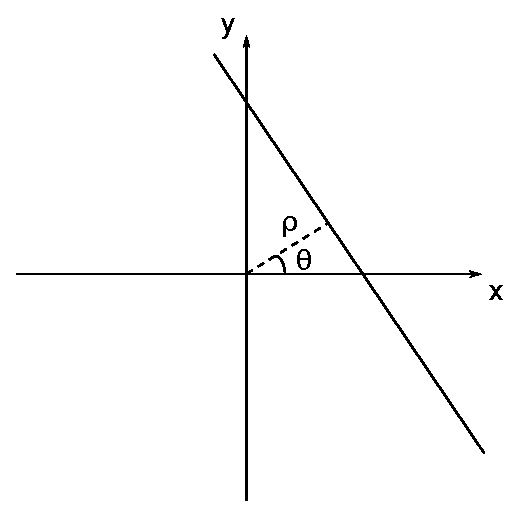
\includegraphics[scale=0.6]{img/param.eps}
\caption{Parameterisation of a straight line, $x \cos \theta + y \sin \theta = \rho$}
\label{param}
\end{figure}
Once a set of projections have been acquired for various values of $\rho$ and $\theta$ (spanning $180^{\circ}$ or $360^{\circ}$), one may intuitively expect that by smearing the projections along the line of the path of the imaging particle on to the reconstruction region, known as \textit{back projection}, the original image function can be reproduced. With this approach, for each angle $\theta$, the image formed by back projection is given by 
\begin{equation}
b(x,y, \theta) = g(x \cos \theta + y \sin \theta, \theta) 
\end{equation}
By integrating over all back projections, the reconstructed image is obtained,
\begin{equation}
f(x,y) = \int_0^\pi b(x,y,\theta) d\theta
\end{equation}
However, this produces image functions that suffer from blurring of the original image, not accurate enough for use in medical CT. For this reason, the filtered back projection method consists of two stages: 1) filtering of the projection data, which will be introduced alongside the Fourier slice theorem in the next section, and 2) back projection of the filtered data.

\subsubsection{Fourier slice theorem}
Consider the projections, $g(\rho, \theta)$ for which the projection angle $\theta$ is fixed. The 1D Fourier transform with respect to $\rho$ is
\begin{equation}
G(\omega, \theta) = \int_{-\infty}^{+\infty}g(\rho, \theta) e^{-i 2\pi \omega \rho} d\rho
\end{equation}
Replacing $g(\rho, \theta)$ with the Radon transform in equation \ref{radon} and rearranging the order of integration,
\begin{align}
G(\omega, \theta) &= \int_{-\infty}^{+\infty}\int_{-\infty}^{+\infty}f(x,y) \left[\int_{-\infty}^{+\infty}\delta(x \cos \theta + y \sin \theta - \rho) e^{-i 2 \pi \omega \rho}d\rho\right]dx dy \\
& = \int_{-\infty}^{+\infty}\int_{-\infty}^{+\infty} f(x,y) e^{-i 2 \pi (\omega x \cos \theta + \omega y \sin \theta)} dx dy \label{G}
\end{align}
where the property of the $\delta$ function was applied to eliminate the integral with respect to $\rho$. By making the replacements $ u = \omega \cos \theta$ and $v = \omega \sin \theta$, it becomes apparent that equation \ref{G} is simply the  2D Fourier transform, $F(u,v)$, of the image function $f(x,y)$,
\begin{equation}
F(u,v) = \int_{-\infty}^{+\infty}\int_{-\infty}^{+\infty} f(x,y) e^{-i 2 \pi (ux + vy)} dx dy
\label{f2d}
\end{equation}
Thus it can be concluded that the 1D Fourier transform of the projection at an angle $\theta$ is equal to a slice of the 2D Fourier transform, $F(u,v)$, of $f(x,y)$, parallel to the projection line: $F(u,v) = G(\omega, \theta)$.

%To find the function $f(x,y)$ through inversion of equation \ref{f2d} (or equivalently equation \ref{G}),
The function $f(x,y)$ is deduced through the inverse Fourier transform of equation \ref{f2d}
\begin{equation}
f(x,y) =  \int_{-\infty}^{+\infty}\int_{-\infty}^{+\infty} F(u,v) e^{i 2 \pi (ux + vy)} du dv
\end{equation}
The integral can be reformulated using polar coordinates, where $du dv = \omega d\omega d\theta$,
\begin{align}
f(x,y) & =  \int_{0}^{2\pi} \int_0^{+\infty} F(u, v) e^{i 2\pi (x \cos \theta + y \sin \theta) \omega } \omega d\omega d\theta \\
& =  \int_{0}^{\pi} \int_{-\infty}^{+\infty} |\omega |G(\omega, \theta) e^{i 2\pi \rho \omega} d\omega d\theta 
\label{fbp}
\end{align}
In the above equation, the filtering stage is performed by multiplying the Fourier transform of the projection, $G(\omega, \theta)$, by $| \omega  |$, and the back projection step is the inverse Fourier transform of $|\omega|G(\omega, \theta)$.

Thus the filtered back projection consists of four steps:
\begin{enumerate}
\item Compute $G(\omega, \theta)$, the 1D Fourier transform of each projection angle uniformly distributed about $180^{\circ}$
\item Filter each 1D Fourier transform by multiplying by $| \omega |$
\item Take the 2D inverse Fourier transform of $F(u,v)$
\item Integrate over all angles to find $f(x,y)$
\end{enumerate}

\subsubsection{Application of FBP to Proton CT}
\label{fbpapp}
Though the filtered back projection method demands rectilinear and parallel particle tracks\footnote{Commonly, non-parallel tracks are transformed to parallel tracks through a reweighting and interpolation procedure - see chapter 3 in \cite{avinash1988principles} }, various attempts have been made at applying the FBP method for proton CT. The following articles reconstructed 2D slices of phantom objects using data obtained through Monte Carlo simulations.
%Based on the measurements of entering and exiting proton positions and energies, authors have imposed strict cuts on protons deviating excessively from a straight path. 

Cirrone et al \cite{cirrone2011monte} investigated the spatial and relative electron density resolution (recall that the WEPL $\approx$ relative electron density, see section \ref{sec:WEPL}) using two different methods to filter protons that deviated excessively from a straight path. The phantom was divided into 1 mm channels. The first method eliminates from the reconstruction protons that enter the reconstruction region through one channel and exit through another. This method, however, does not take into consideration the path inside the phantom. The second exclusion criteria uses the most likely path formalism (see section \ref{pathformalism}): any proton whose most likely path trajectory exits its incident channel is removed from the reconstruction. The authors were able to obtain a relative electron density resolution of approximately 1.1 \%, almost reaching the desired $< 1\%$ resolution of proton CT. However, spatial resolution was limited to 3 mm whereas the desired proton CT spatial resolution is $<$ 1 mm. A similar method was used in \cite{aso2007study}, demanding that the lateral displacement between ingoing and outgoing proton positions was less than 1 mm.

A distance-driven binning approach for FBP using most likely paths has also shown to improve spatial resolution relative to the standard FBP method, without any loss to density resolution \cite{rit2012distance}. However, the resolution was not quantified to be able to compare with other methods.

A \textit{backprojection-then-filtering} method, which the authors claim to naturally accommodate the curved path trajectory of protons, was used to reconstruct images in \cite{poludniowski2014proton}. The study demonstrated a relative stopping power accuracy of $\approx 0.1\%$. However, water at a variety of densities was the only media investigated and subsequent simulations are needed to study the method using a mixture of realistic tissue compositions.

Simulations evaluating the effect of FBP on density resolution were performed by Schulte et al \cite{schulte2005density}. They achieved a relative stopping power accuracy of $\approx 1\%$ at the centre of a cylindrical 20 cm diameter phantom.

The PRIMA (PRoton IMAging) collaboration have published preliminary results using data acquired from their proton CT apparatus using tracking detectors \cite{vanzi2013prima}. With FBP they were able to obtain a spatial resolution of 0.88 mm and 2.5\% density accuracy.

\subsection{Algebraic Reconstruction Techniques}
For certain imaging situations it is difficult or not possible to obtain a full set of projection data, possibly due to limitations in the size of the scanners or due to the size of large objects. In such cases a branch of iterative algorithms can be used, the most well known of which is the algebraic reconstruction technique (ART). Unlike FBP, for which a uniformly distributed set of projection data over $180^{\circ}$ or $360^{\circ}$ is required, ART is able to reconstruct an image from limited views.

The formulation of ART is simpler and more flexible than the analytical FBP approach, and permits a priori knowledge to be used in the reconstruction. Initially, one may believe that this would be the most appropriate and hopeful approach to proton CT as information about the proton path can be incorporate into the algorithm (see section \ref{pathformalism}). However, ART methods suffer from slow reconstruction times and large computational costs. With increasingly powerful CPUs and the advances in GPU technology, reconstruction speeds have increased significantly and the times required for proton CT reconstruction is becoming increasingly attainable.

\subsubsection{Image projection}
As was explained in \ref{sec:fbp}, the reconstruction region is represented as a function of position, $f(x,y)$. By superimposing a grid of $N$ cells, as shown in figure \ref{fig:grid}, it can be assumed that $f(x,y)$ is constant in each cell, and the value of the $j^{th}$ cell is $f_j$, where $j = 1 \ldots N$. Thus the projection $p_{i}$ of the $i^{th}$ ray can be expressed as
\begin{eqnarray}
p_{i} = \sum_{i}^N w_{ij} f_j
\label{proj}
\end{eqnarray}
\begin{figure}[h]
\centering
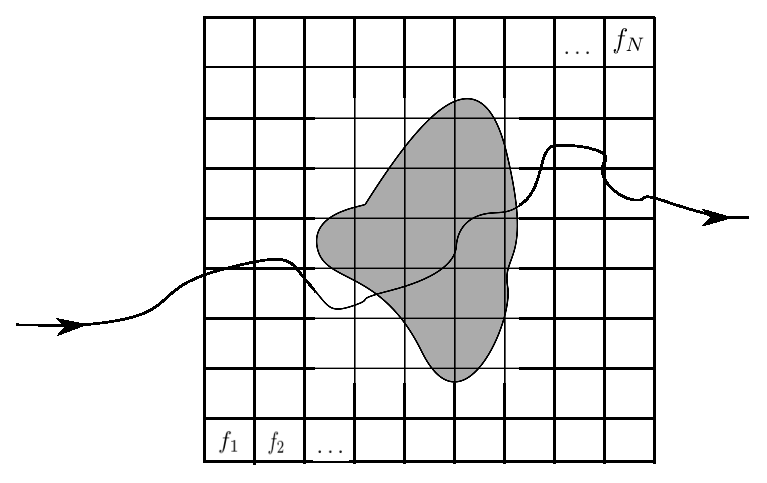
\includegraphics[scale=0.8]{img/grid.eps}
\caption{The reconstruction region $f(x,y)$ is discretised into a grid of cells $f_j$, where $j = 1 \ldots N$. The grey shaded shape represents a volume being imaged. The arrow shows a possible path a proton may take through the reconstruction region.}
\label{fig:grid}
\end{figure}
where $i = 1 \ldots M$, $M$ is the total number of projections and $w_{ij}$ is a matrix of weighting factors, called the \textit{system matrix}, giving the contribution of the $j^{th}$ cell to the $i^{th}$ ray projection. The weighting factor can be chosen as the length of the $i^{th}$ ray through $j^{th}$ cell. For images of size $256 \times 256$, $N$ is of the order of $10^{4}$, and generally $M$ is of the same order. The matrix $w$ is thus large and has dimensions $10^{4} \times 10^{4}$ making direct matrix inversion infeasible to obtain $f_{j}$. It was Kaczmarz in 1937 who first proposed an iterative method to find $f_{j}$ through his "method of projections" \cite{kaczmarz1937angenaherte}.

Consider the projections in equation \ref{proj} in their expanded form,
\begin{equation}
\begin{aligned}
w_{11}f_{1} + w_{12}f_{2} + \ldots + w_{1N} f_{N} & =  p_{1} \\
w_{21}f_{1} + w_{22}f_{2} + \ldots + w_{2N} f_{N} & =  p_{2} \\
\vdots \\
w_{M1}f_{1} + w_{M2}f_{2} + \ldots + w_{MN} f_{N} & =  p_{M} 
\label{planes}
\end{aligned}
\end{equation}
The cell values (i.e. the image) can be written in a compact vector form in an $N$ dimensional space as $\vec{f} = (f_{1}, f_{2}, \ldots, f_{N})$ and each projection in equation \ref{planes} can be considered as a hyperplane in this space. If a unique solution exists (which would be the case for an ideal system) then all the hyperplanes intersect at the single point $\vec{f}$.

The vector $\vec{f}$ can obtained through an iterative procedure through the following,
\begin{equation}
f_{j}^{(i)} = f_{j}^{(i-1)} + \frac{p_i - q_i}{\sum_{k=1}^N w_{ik}^2}
\label{ART}	
\end{equation}
where
\begin{equation}
q_{i} = \vec{f}^{(i-1)} . \vec{w}_{i} = \sum_{k=1}^N f_{k}^{(i-1)}w_{ik}
\end{equation}
and $f_{j}^{(i)}$ is the $j^{th}$ component of $\vec{f}$ on the $i^{th}$ iteration. Each iteration is equivalent to the projection of the vector $\vec{f}^{(i-1)}$ onto the $i^{th}$ hyperplane in equation \ref{planes} to obtain $\vec{f}^{(i)}$. An initial guess must be chosen for $\vec{f}^{(0)}$. It has been shown that if a unique solution $\vec{f}_{s}$ exists to the system of equations in (\ref{planes}) then the iterative procedure is guaranteed to converge \cite{tanabe1971projection},
\begin{equation}
\lim_{k \to \infty} \vec{f}^{(k)} = \vec{f}
\end{equation}
It should also be noted that, as is often the case, there are more projections than there are cells in the reconstructed image - that is, $M > N$ - and the projections $p_i$ are corrupted by noise. Thus equations (\ref{planes}) form an overdetermined system and no unique solution to $\vec{f}$ exists. The iterative procedure will thus oscillate in the neighbourhood of the intersection of the planes.

We refer the reader to \cite{avinash1988principles} for a more descriptive introduction to ART and the construction of equation (\ref{ART}), as well as its various implementations (SART, SIRT).

\subsubsection{Application of ART to proton CT}
The ART method and its various forms have been used in the literature and generally it is assumed that this approach can provide a better spatial resolution and proton stopping power accuracy than that obtained through the FBP method. Nothing in the literature was found that directly compared both ART and FBP algorithms and their variations applied to proton CT data for the same phantom. However, a combination of FBP used to initialise the initial guess in ART has been used \cite{penfold2009characteristics}. The iterative method to image reconstruction has been used in medical imaging long before the recent surge in interest in proton therapy. Recent advances in computer power and memory have helped overcome some of the original limitations. Nevertheless, it is still significantly more time consuming to construct images using ART than FBP.

The biggest advantage of ART over FBP is the ability to incorporate information about the proton path. Schulte et al traced proton trajectories through the reconstruction region using three different estimates of the trajectory of the proton to construct the matrix of weighting factors \cite{li2006reconstruction}. For complex path estimates, constructing the system matrix may be computationally costly and difficult. Penfold et al introduced the concept of an \textit{effective chord length} for all pixel intersections in each proton's trajectory \cite{penfold2009more}.

Application of ART in an experimental set up has been applied to data acquired from a prototype proton CT scanner in \cite{hurley2012water}.

It should be noted that there are far too many variations of ART to include in this review. The interested reader is referred to \cite{penfold2015techniques} for recent developments in ART applied to proton CT.

\section{Proton Path Formalism}
\label{pathformalism}
Due to the elastic multiple coulomb scattering events that deflect the proton from a straight path as it traverses a material, the proton follows a curved trajectory path. In addition to the elastic events, large deflections occur through nuclear inelastic collisions. Though much less frequent than MCS, they lead to large angular scattering events. The majority of these protons will not make it through the reconstruction region, and those that do are typically filtered out from the reconstruction through strict cuts on the outgoing energy of the proton \cite{li2006reconstruction}. 

The unknown trajectory of the protons results in an inherent blur and limitations in spatial resolution in reconstructed images. Various formalisms have been used in an effort to estimate the path of the proton as it passes through a medium. The three most common proton path estimates that are used in the literature are introduced below. A comparison of the straight line path, most likely path and cubic spline path estimates was performed in \cite{li2006reconstruction}. It was found that the most likely path estimate predicts the path of the proton to the highest degree of precision and results in a faster convergence and higher spatial resolution using ART. 

\subsection{Straight line}
The simplest approach to the path estimation of the proton through a medium is to assume that the proton travels along a straight line connecting the position at which it enters the reconstruction region to the position that it leaves the reconstruction region.

\subsection{Most likely path}
\label{sec:appmlp}
Each MCS event leads to a complex distribution of scattering angles. The combined angular scattering distribution of many MCS events, however, can be approximated as Gaussian \cite{eyges1948multiple}. Similarly, the lateral displacement of the proton can also be approximated as Gaussian distributed. Given these two approximations and taking into account the correlation between scattering angle and lateral displacement a proton, the statistically most likely trajectory of a proton can be determined given the trajectory's entry and exit angle and position in the medium. The path can be considered as the best statistical estimate of a proton through a medium. For brevity, the mathematical formalism for the most likely path (MLP) is omitted here, but the reader is directed to \cite{williams2004most,schulte2008maximum} for the derivation. 


\subsection{Cubic spline path}
\label{sec:spline}
A mathematically simpler estimation of the proton path that incorporates curved trajectories is the fitting of a cubic spline to the endpoints of the proton trajectory. The path of the proton can be estimated as 
\begin{equation}
t(u) = a + b u + c u^2 + d u^3
\end{equation}
where $t$ is the lateral deflection at a depth $u$. The coefficients $a$, $b$, $c$ and $d$ can be determined by fitting the cubic polynomial to the beginning and endpoint location and slope of the proton trajectory.

\section{Conclusion}
Treatment planning uncertainties resulting from conventional x-ray scans can lead to errors in the proton range of the order of 2-3 mm. Furthermore, patient verification in the treatment room is routinely performed using x-ray cone beam CT. Proton CT has the potential of measuring more accurately the stopping power of protons in a medium as well as providing a means of pretreatment set up verification. The underlying physical interactions of protons as they traverse a medium and the straggling of protons have been discussed. The Water Equivalent Path Length (WEPL) has been introduced, and it has been shown how it relates to the stopping power of protons relative to water. The filtered backprojection method (FBP) and algebraic reconstruction technique (ART) have been reviewed, and a brief overview of results obtained in the literature has been given. 
\bibliographystyle{ieeetr}
\bibliography{bibfile}{}
%\bibliographystyle{unsrtnat}

\includepdf[pages={2}]{kthcover.pdf}
\end{document}

\end{document}